\documentclass{article}

\usepackage{float} % formatting figures
\usepackage{graphicx} % for figures
\usepackage{caption} % for continuing figures

\usepackage{arxiv}
\usepackage[utf8]{inputenc} % allowhttps://www.overleaf.com/project/5c87bf080afdb00df417c5e7 utf-8 input
\usepackage[T1]{fontenc}    % use 8-bit T1 fonts
\usepackage{hyperref}       % hyperlinks
\usepackage{url}            % simple URL typesetting
\usepackage{booktabs}       % professional-quality tables
\usepackage{amsfonts}       % blackboard math symbols
\usepackage{nicefrac}       % compact symbols for 1/2, etc.
\usepackage{microtype}      % microtypography
\usepackage{lipsum}

\usepackage{amsmath}
\usepackage{amssymb}

\title{Simulating Rayleigh-Bénard Convection on Harvard Odyssey}


\author{
   Jiawei Zhuang \\
   Harvard University\\
   \textit{jiaweizhuang@g.harvard.edu}\\
   \And
   Yiqi Xie \\
   Harvard University \\
   \textit{yiqi\_xie@g.harvard.edu}\\
   \And
   David Pineiro \\
   Harvard University \\
   \textit{davidpineiro@g.harvard.edu}\\
}
  %% \AND
  %% Coauthor \\
  %% Affiliation \\
  %% Address \\
  %% \texttt{email} \\
  %% \And
  %% Coauthor \\
  %% Affiliation \\
  %% Address \\
  %% \texttt{email} \\
  %% \And
  %% Coauthor \\
  %% Affiliation \\
  %% Address \\
  %% \texttt{email} \\

\begin{document}
\maketitle


\section{Introduction}

In this report, we consider the Rayleigh-Bénard convection (RBC), which corresponds to the flow of a fluid placed between two horizontal surfaces, the top which is cold and the bottom one hot, in a gravitational field perpendicular to surfaces pushing downward. To better understand the dynamics of this problem, we will first discuss thermal convection, followed by introducing the tool we used to simulate and solve this computationally expensive problem.

\subsection{Thermal Convection}
Thermal convection is a natural process that drives fluids in motion. This phenomenon occurs when thermal energy is transferred from one location to another by the movement of fluids. There exits two general kinds of thermal convection: natural convection and forced convection. The former occurs when fluids are driven in motion by buoyancy forces, which are affected by changes in density caused by the surrounding temperature. The particles near a hot surface become excited, thus scattering and causing the fluid to be less dense, while the particles near the cold surface sink. Therefore, causing the hotter volume to transfer heat towards the cooler volume of that fluid. This interaction between the varying densities leads to various fluid dynamics, which we observe in our simulation. On the other hand, there exists forced convection, which occurs when a fluid is forced to flow over the surface by an internal source such as fans and pumps, creating an artificially induced convection current. This report will focus on natural convection. 

Thermal convection has many applications, and understanding its dynamics is vital in understanding the the nature of the universe we live in. Researchers have been trying to understand the mechanics of this naturally occurring phenomenon for quite some time. Henri Claude Bénard in 1900 observed a fluid behaving in an atypical fashion on a Petri dish placed on a hot plate. Although, Bénard's setup was a result from surface tension effects, it was only years later that a British mathematician, Lord Rayleigh successfully determined under what conditions this thermal convection occurred. 

Since then, because of the prevalence of thermal convection, it has been at the center of many research studies. In 1978, an article was published in the Journal of Agricultural Engineering Research by JM Bruce, shedding light into cattle ventilation [1]. By studying the various geometries and relevant to buildings, Bruce developed a theory which lead to design procedures for open-ridge and slotted-roof systems of ventilation for cattle buildings. This example highlights the importance of understanding thermal convection and its impact in our everyday lives. 


\subsection{Harvard Odyssey}
The Harvard Odyssey is high performance computing cluster, commonly known as HPC cluster. Odyssey is commonly used for scientific modeling and simulation of a significant percentage of Harvard researchers. Using a SLURM task manager, Odyssey allocates various requested resources from its nodes with 8 to 64 cores and from its 1,000,000 NVIDIA GPU cores.

Additionally, with over 35 petabytes of memory, Odyssey has two underlying networks for computational efficiency. The first is a traditional TCP/IP network and the second is a low-latency 56 Gb/s FDR InfiniBand network that enables high-throughput messaging for parallel-computing and fast access memory. Odyssey also maintains thousands of compiled software libraries available to its users. 

To perform the computation needed for this project, we utilized various resources provided by Odyssey, along with a Sandia Labs-provided implementation for Drekar, a highly-reliable partial differential equations for fluids solver. We discuss Drekar in the following section.
% TODO: aspect ratio
% TODO: time steps
% TODO: finite elements

\section{Description of Code}

As mentioned in the previous section, Drekar is a large scale computational fluid dynamics and electromagnetic partial differential equations (PDE) solver. Using parallel finite element code written in C++, it uses various algorithms and numerical methods to solve PDEs. A fundamental asset of Drekar is that it is was built on Trilinos, a centralized library of various highly efficient computational packages. In fact, Trilinos is a Greek term for “string of pearls,” meant to symbolize the importance of the other packages it carries, while being a pearl itself. 

Drekar requires an .xml input file in which all of the parameters, methods, constraints, and tools to solve a problem are specified. 

ParameterList Structures in XML file: 

\begin{itemize}
    \item[] \textbf{<ParameterList name = 'Mesh'>:} We begin the input file by setting and specifying the mesh, which can be either imported from an Exodus file, or specified. The mesh is also where we specify certain boundary conditions such as periodicity, although the rest of the boundary conditions is made into its own ParameterList Structure. 
    \item[] \textbf{<ParameterList name = 'Physics Blocks'>:} After setting up the mesh structure, we set up physics blocks. These blocks establish environments where specific variables will be used in the equations Drekar will try to solve. Also, these blocks allow us to specify finite element methods, their parameters, and stabilization information. These blocks are later referenced boundary conditions are specified.
    \item[] \textbf{<ParameterList name = 'Boundary Conditions'>:} These contain references to the behavior of the constraints, as well as pointers to where in the problem setup it belongs. 
    \item[] \textbf{<ParameterList name = 'Closure Models'>:} This structure helps Drekar evaluate the parameters we are interested in and output them accordingly, as specified by the Output structure below.
    \item[] \textbf{<ParameterList name = 'Output'>:} This structure helps Drekar redirect its output to a file specified in this structure.
    \item[] \textbf{<ParameterList name = 'Solver Factories'>:} Used to specify Drekar's output granularity. That is, how often it writes to the output file.  
\end{itemize}
 
 Using these XML structures we were able to set up the Rayleigh-Bénard convection problem with specific parameter values specified in section 4.


% Show that you understand the xml file
% Trilinos
% https://trilinos.org/docs/files/TrilinosOverview.pdf
% in class slides

\section{Numerical Methods Utilized}
\subsection{Spatial Discretization}
The spatial part of the PDE problem is handled with the Finite Element Method (FEM). The essential idea of FEM is to first derive the weak form of the original problem, then represent the weak form using a set of functional basis defined on the discretized space elements, and in the end solve the problem under the new representation. 

Here we take the example provided by T. J. R. Hughs in his \emph{The Finite Element Method}, sect 1.12 - 1.15. We start with an 1D Poisson equation with boundary conditions:
\begin{align}
    -\partial_x^2 u=f(x),&\quad x\in(0,1), \\
    -\partial_x u(0)=\mathfrak{h},&\quad u(1)=\mathfrak{g}.
\end{align}
The weak form says to find $u\in\mathcal{S}$, \emph{s.t.} $\forall w\in\mathcal{V}$,
\begin{align}
    \int_0^1\!\partial_x w\partial_x u~\mathrm{d}x
    =\int_0^1\! w f~\mathrm{d}x + w(0)\mathfrak{h}.
\end{align}
We discretize the $x$ domain by $n$ elements \begin{align*}
    \begin{gathered}
        (x_1,x_2),~(x_2,x_3),~\ldots,~(x_n, x_{n+1})\\
        \mathrm{where}~x_1=0,~x_{n+1}=1
    \end{gathered}
\end{align*}
and choose the functional basis to be
\begin{align}
    N_i(x)=\left\{\begin{aligned}
        &\frac{x-x_{i-1}}{x_i-x_{i-1}}&,&\quad x\in(x_{i-1},x_i]\\
        &\frac{x_{i+1}-x}{x_{i+1}-x_i}&,&\quad x\in(x_{i},x_{i+1}]\\
        &0&,&\quad \mathrm{elsewhere}
    \end{aligned}\right.
    ,\quad i=1,2,\ldots,n+1. \\
\end{align}
The weak form can now be written in the discretized form, \emph{i.e.} the Galerkin statement
\begin{align}
    \int_0^1\!\partial_x w^h\partial_x u^h~\mathrm{d}x
    =\int_0^1\! w^h f~\mathrm{d}x + w^h(0)\mathfrak{h},
\end{align}
where the functions should be represented by
\begin{align}
    u^h=\sum_{i=1}^nu_iN_i+\mathfrak{g}N_{n+1},\quad
    w^h=\sum_{i=1}^nw_iN_i.
\end{align}
This gives us the equation for the coefficients $u_i$ and $w_i$
\begin{align}
    \sum_{i=1}^n w_i \left(\sum_{j=1}^n K_{ij} u_{j} - F_i\right)=0,\label{eqn:weak_dis}
\end{align}
where
\begin{align}
    K_{ij}=\int_0^1\!\partial_xN_i\partial_xN_j~\mathrm{d}x,\quad
    F_i=N_i(0)\mathfrak{h}+\int_0^1\!N_if~\mathrm{d}x-\mathfrak{g}\int_0^1\!\partial_xN_i\partial_xN_{n+1}~\mathrm{d}x
\end{align}
are known to us. Note that the weak form should work for any $w$, thus from (\ref{eqn:weak_dis}) we must have
\begin{align}
    \sum_{j=1}^n K_{ij} u_{j} - F_i=0, 
\end{align}
which is a linear equation system whose solution gives us the $u$ we want. 


\subsection{Temporal Discretization}
The temporal part of the PDE is handled by the SDIRK method, a member of the implicit Runge-Kutta family. The implicity helps to keep the numerical solution stable. 

\subsection{Non-linear Solver}
The S-N equation is non-linear. The solver responsible for this part is line-search based, which means a direction for solution update will first be determined and the length of the step moving towards that direction will be then estimated. Here the determination of the direction is achieved using the Newton method. 

\section{Simulation Parameters}
\subsection{The Physical Constants}
The physical system is an infinite slab of fluid confined between two parallel plates that hold a temperature difference, with gravity acting in the downward direction. In the simulation the fluid was set up with the following parameters:
\begin{itemize}
    \item density: $\rho=1$
    \item viscosity: $\mu=10^{-2}$
    \item thermal conductivity: $\kappa=10^{-2}$
    \item volume expansion coefficient: $\alpha_V=10^6$
\end{itemize}
We let the gravity be a unit force acting along the $-y$ direction, and placed the plates at $y_\mathrm{bot}=0$ and $y_\mathrm{top}=1$. The bottom plate was heated up to $T_\mathrm{bot}=1$, while top plate was kept cool at $T_\mathrm{top}=0$. It gave us:
\begin{itemize}
    \item channel height: $H=1$
    \item temperature difference: $\Delta T=1$
    \item gravitational constant: $g=1$
\end{itemize}
So in terms of non-dimensionalization the system was characterized by:
\begin{itemize}
    \item Rayleigh number: $Ra=10^{10}$
    \item Prandtl number: $Pr=1$
\end{itemize}

\subsection{The Boundaries and the Initial State}
For the velocity field, no-slip boundary conditions were assumed on both plates, \emph{i.e.}
\begin{equation}
    \mathbf{u}\big|_{y=0}=0,\quad \mathbf{u}\big|_{y=1}=0.
\end{equation}
The plate temperature is supposed to be static over the simulation time. In practice, however, we ramp the bottom-plate temperature up from $0$ to $1$ in a relatively short time at the beginning of the simulation - this helps to get rid of the meta-stable solution of a thermal-conducting-only fluid. In specific, the temperature boundary conditions were designed as follows:
\begin{equation}
    T\big|_{y=0}=1-\mathrm{e}^{-t/0.2},\quad T\big|_{y=1}=0.
\end{equation}

In addition, in order to solve the infinity of the system along the $x$ direction, we set up a pair of ``artificial'' boundaries at $x_\mathrm{left}=0$ and $x_\mathrm{right}=2$ and assumed periodic boundary conditions for both the velocity field and the temperature field for approximation, \emph{i.e.}
\begin{equation}
    \mathbf{u}\big|_{x=0}=\mathbf{u}\big|_{x=2},\quad \partial_x\mathbf{u}\big|_{x=0}=\partial_x\mathbf{u}\big|_{x=2},
\end{equation}
\begin{equation}
    T\big|_{x=0}=T\big|_{x=2},\quad 
    \partial_x T\big|_{x=0}=\partial_x T\big|_{x=2}.
\end{equation}

Finally, the initial conditions were:
\begin{equation}
    \mathbf{u}\big|_{t=0}=0,\quad T\big|_{t=0}=0.
\end{equation}
Note that the initial condition for the temperature field is in accordance to our modification to its boundary condition. 

\subsection{Discretization}
A uniform mesh of $N_x=2048$ was used for the discretization of $x$. To capture the fine structures emerged near the plates, $y$ was discretized with a Chebyshev mesh:
\begin{equation}
    y_i=\frac{1}{2}\left(1-\cos\frac{i\pi}{N_y-1}\right),\quad i=0,1,\ldots,N_y-1,
\end{equation}
where we used $N_y=1024$. 

The time integration was performed with a maximal time step of $10^{-4}$.

\subsection{Computational Resources}
The simulation was performed on Odyssey. The job requested 512 cores with 16GB memory assigned to each. We let it ran for 1 day and the final physical time arrived is $t\approx 0.22$.

\section{Results}

\graphicspath{ {./zhuangjw/img/} }

\subsection{Temperature field}

We first look at the temperature field, which is intuitive and closely related to the heat transfer problem.

\subsubsection{Single-time snapshot}

We choose three time frames to plot: when mushroom-like plumes start to appear; a typical time frame when strong mixing occurs; at the last time step. The video containing all 225 time frames is available in the presentation slides..

\begin{figure}[H]
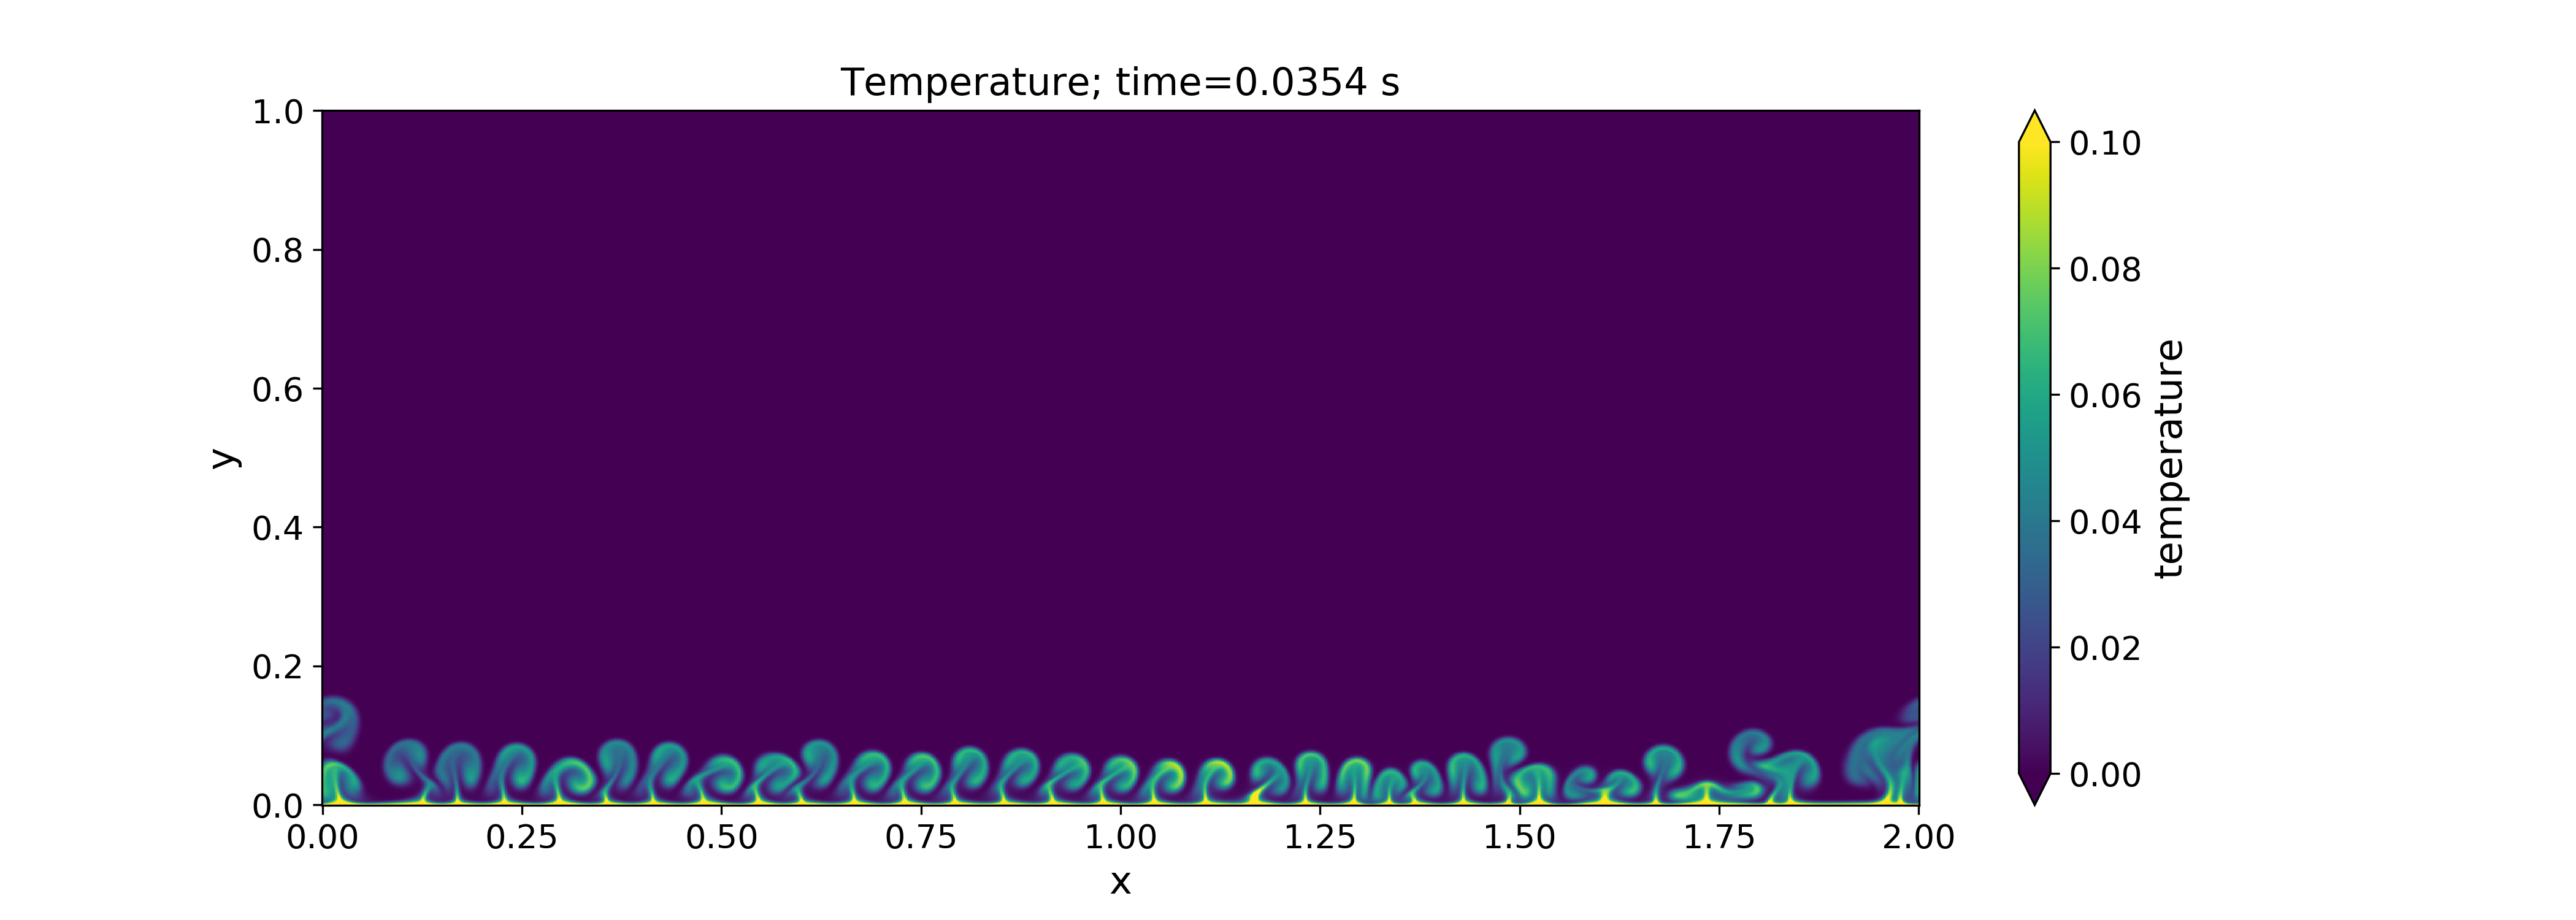
\includegraphics[scale=0.5]{temp_frame_037}
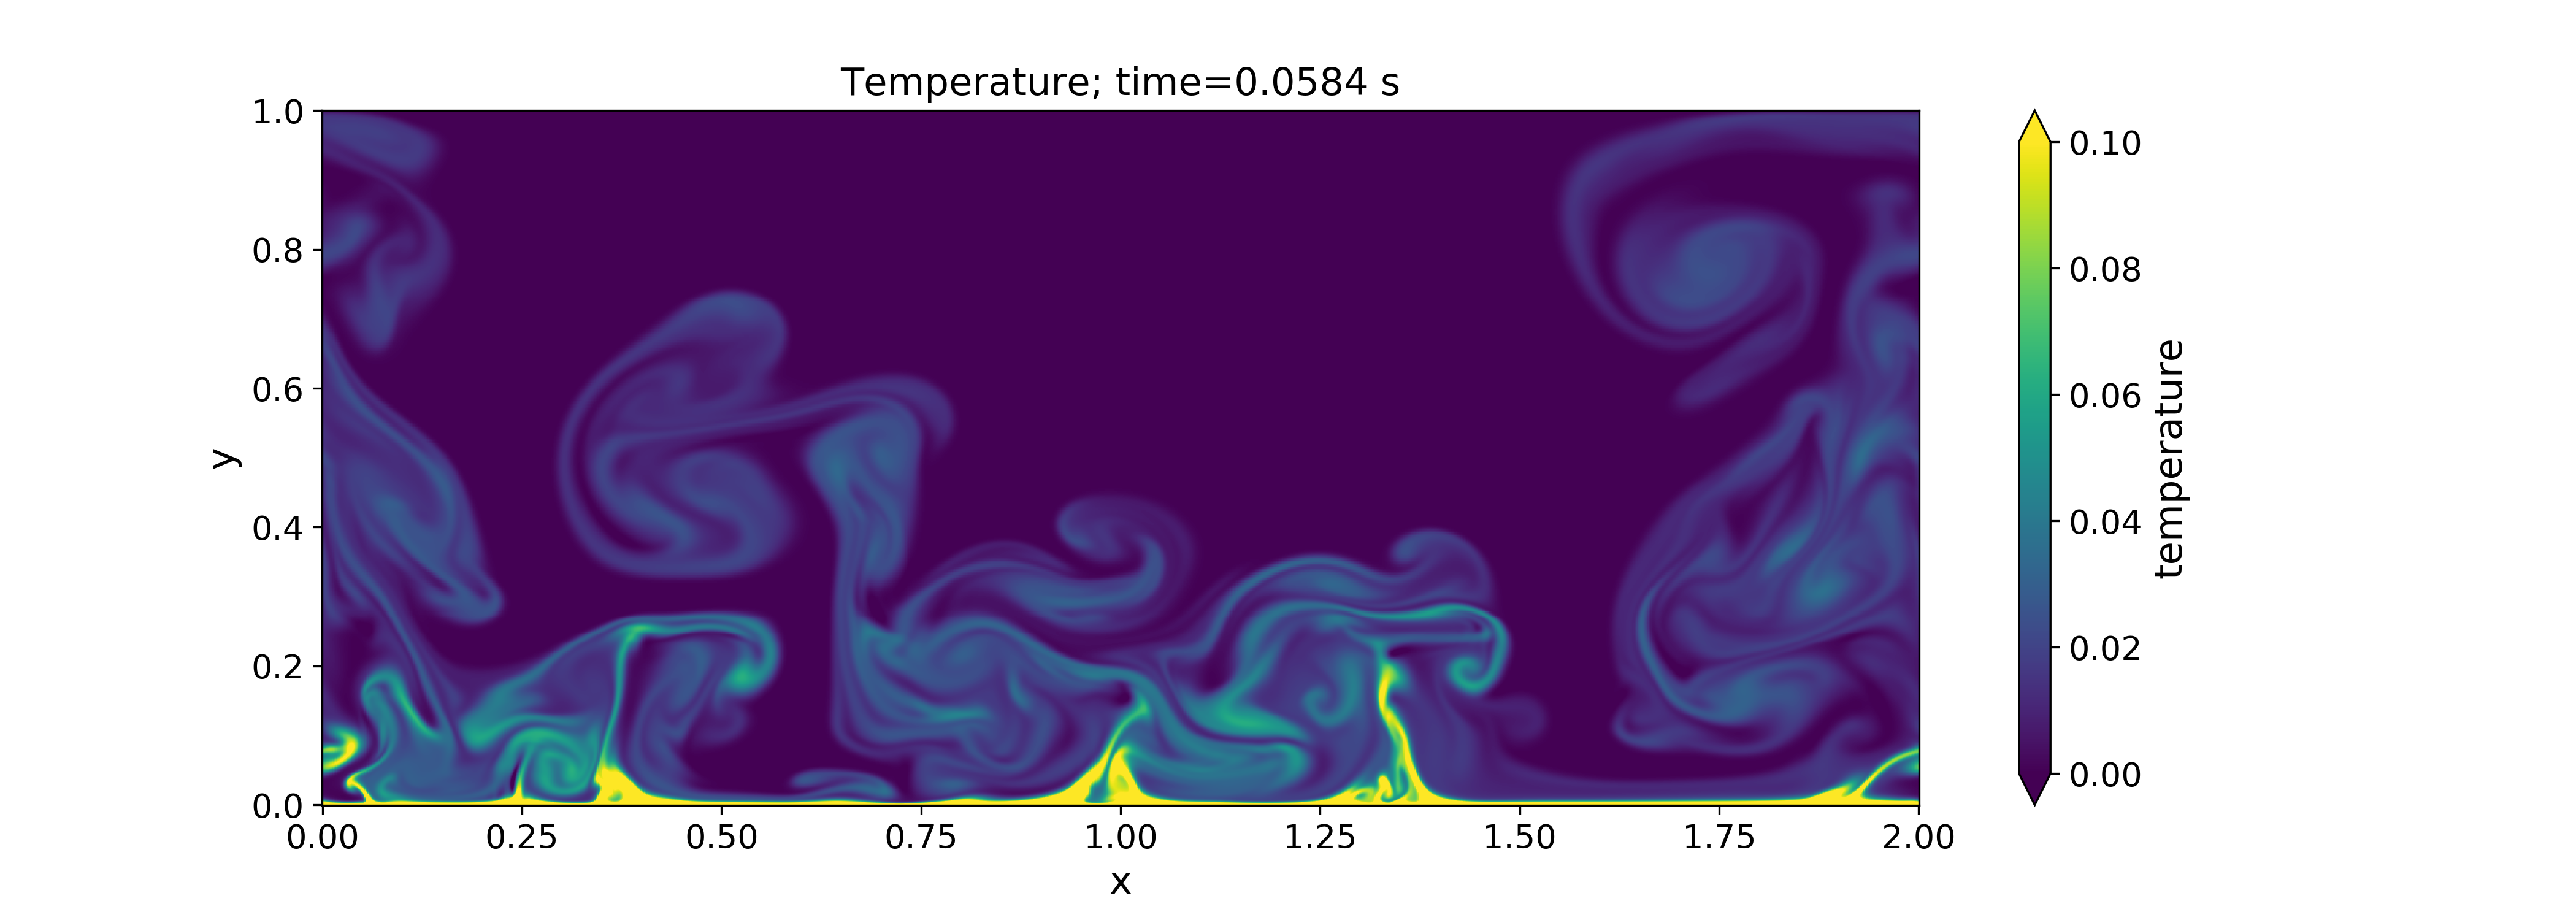
\includegraphics[scale=0.5]{temp_frame_060}
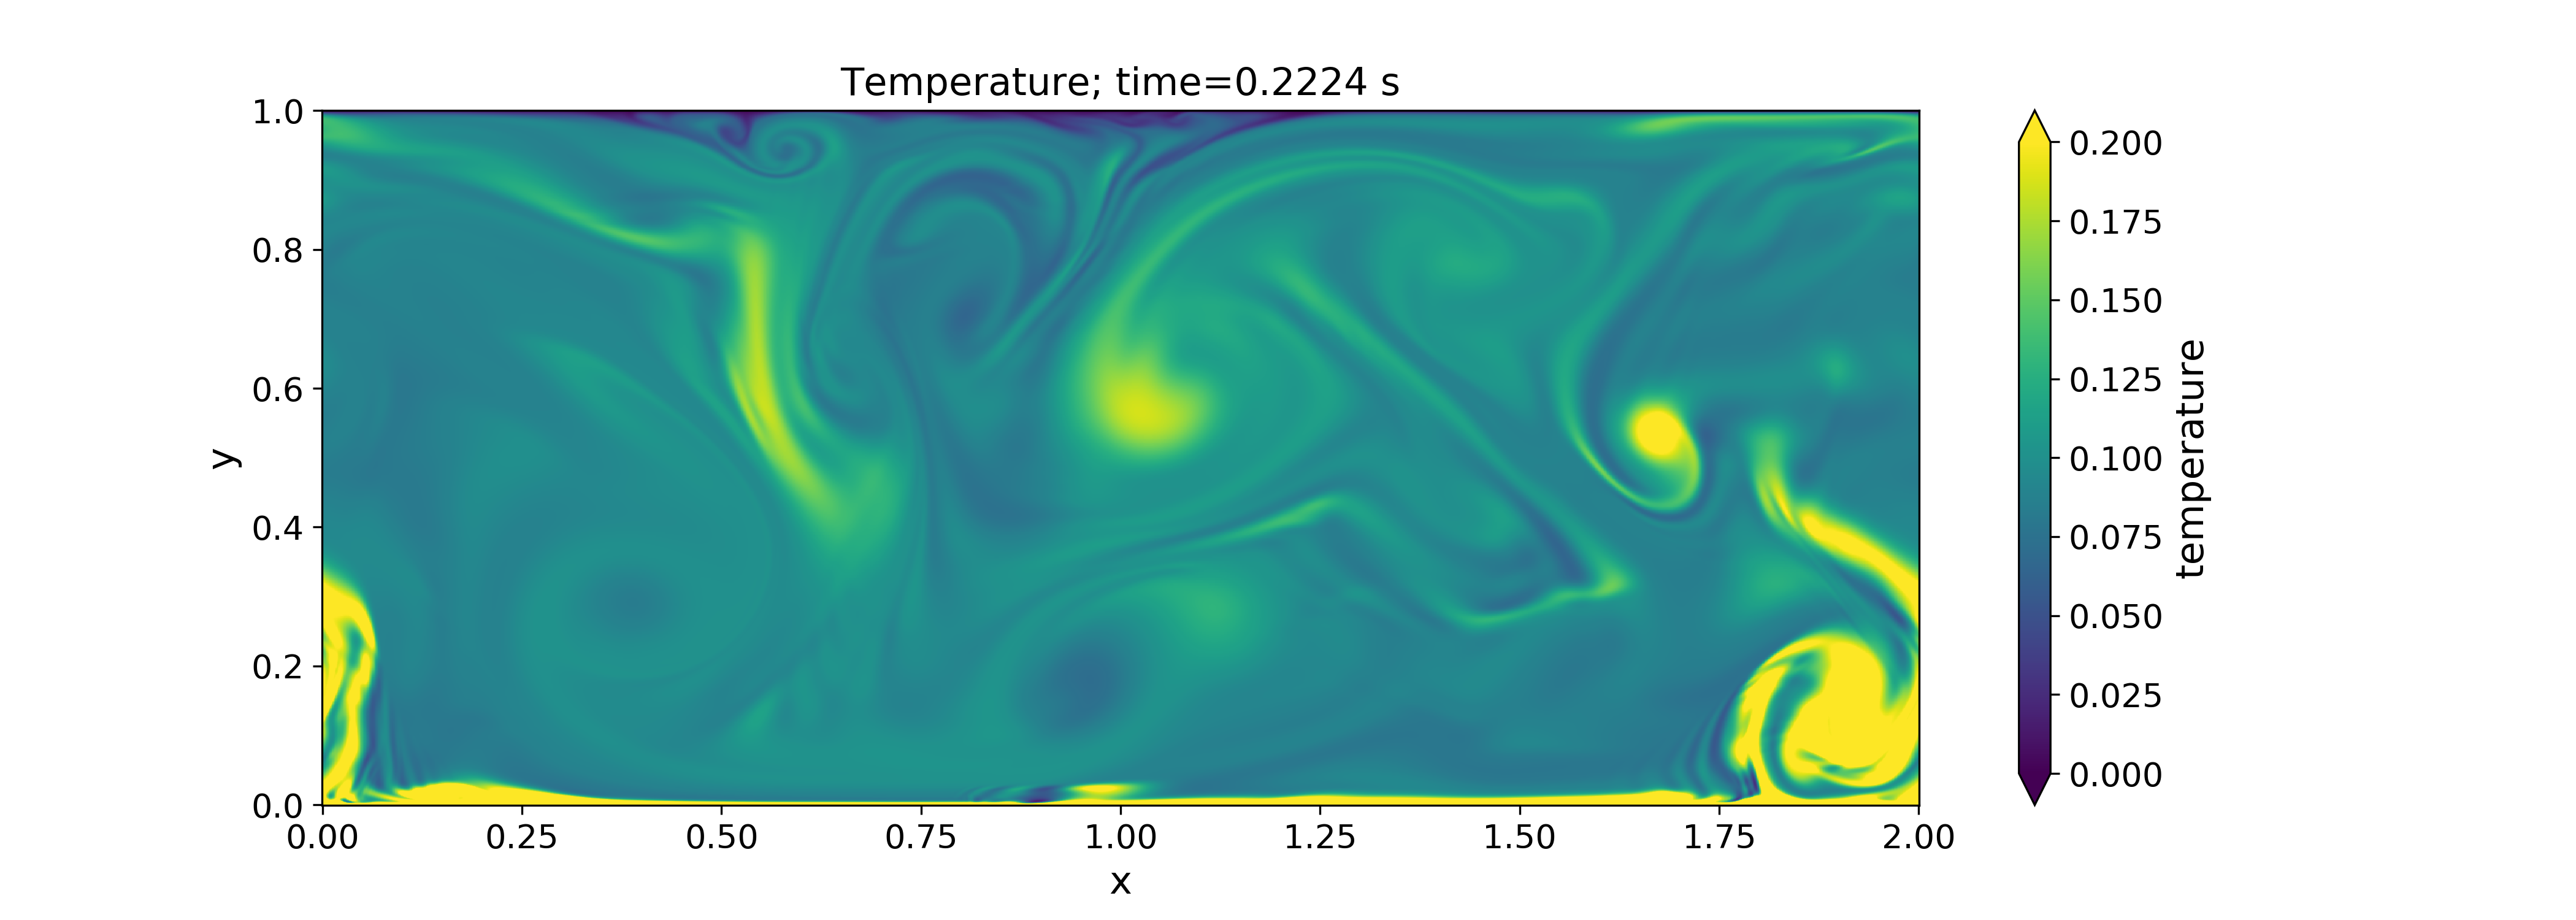
\includegraphics[scale=0.5]{temp_frame_224_vmax02}
\centering
\caption{Temperature field T(x, y) at different time. The last figure has a different colorbar scale, for better visualization.}
\end{figure}

Alternatively, the same temperature field can be plotted with filled-contours. The darkest region are small negative values (around $-10^{-10}$), because we do not cap negative values in the input XML file. Otherwise, the overall pattern is consistent with the previous plot.

\begin{figure}[H]
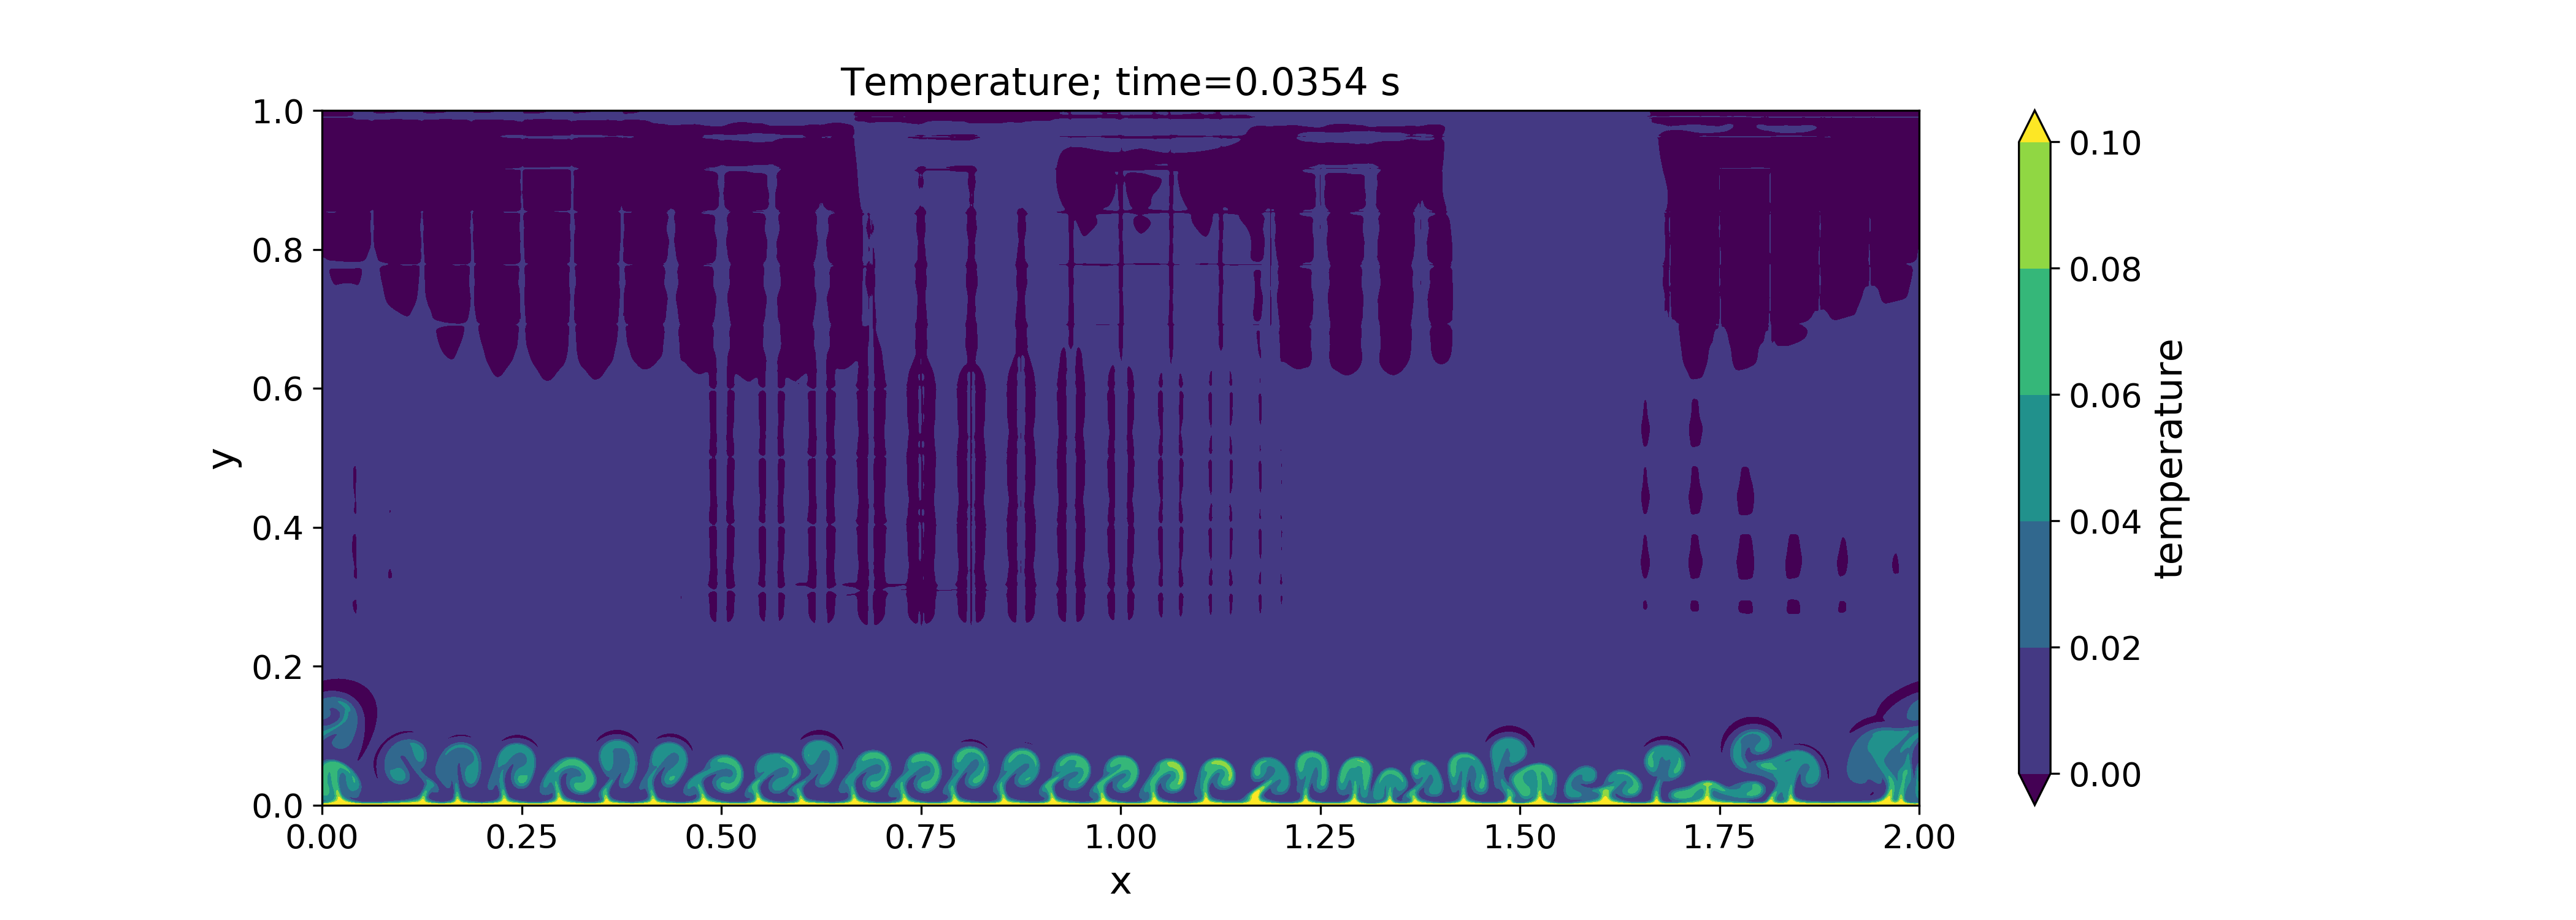
\includegraphics[scale=0.5]{contour_frame_037}
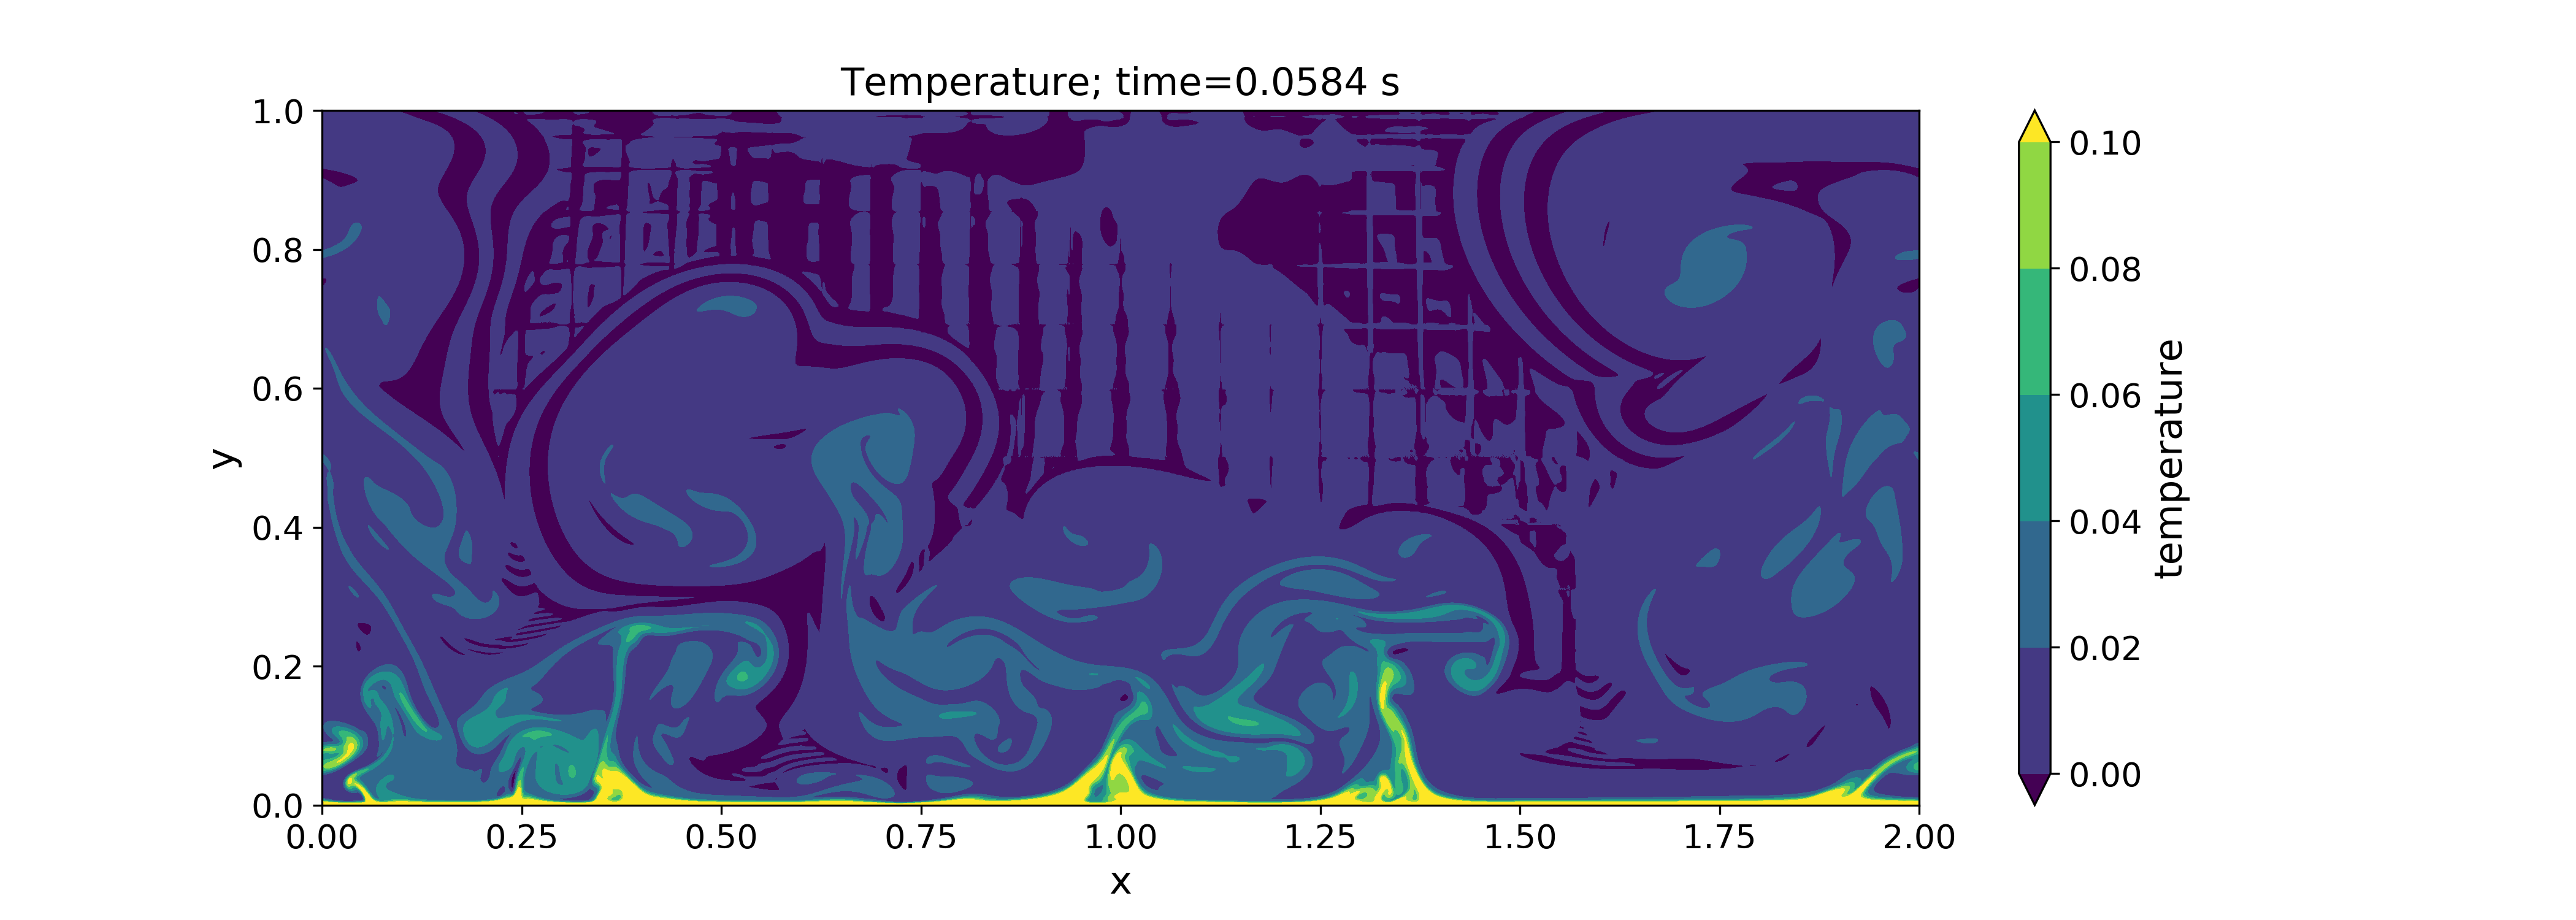
\includegraphics[scale=0.5]{contour_frame_060}
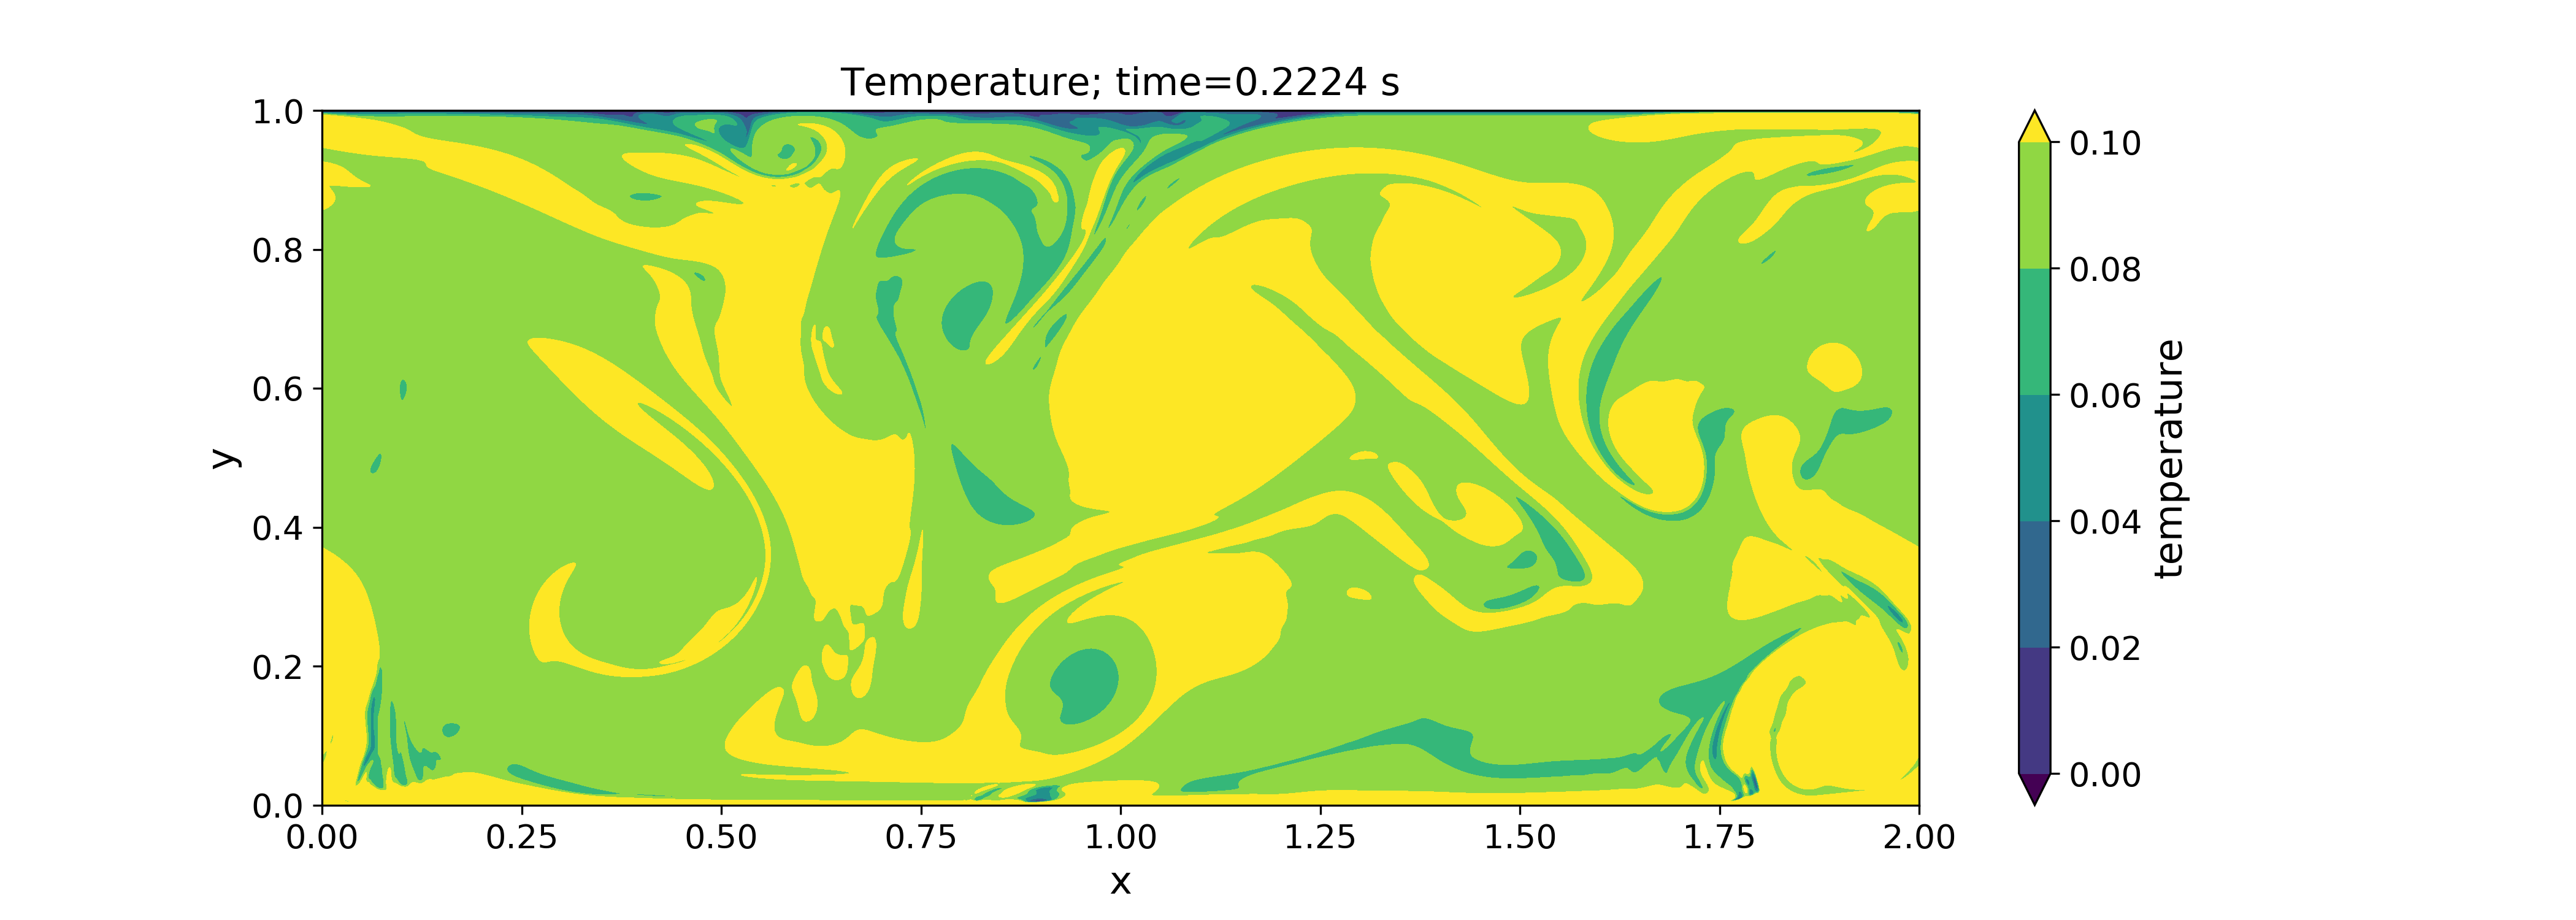
\includegraphics[scale=0.5]{contour_frame_224}
\centering
\caption{Filled-contour plot of temperature field T(x, y) at different time. Darkest regions indicate slight negative values.}
\end{figure}

\subsubsection{Temperature profile}

Then we turn to the vertical profile of temperature. Below shows the temperature profile averaged over x and t.

\begin{figure}[H]
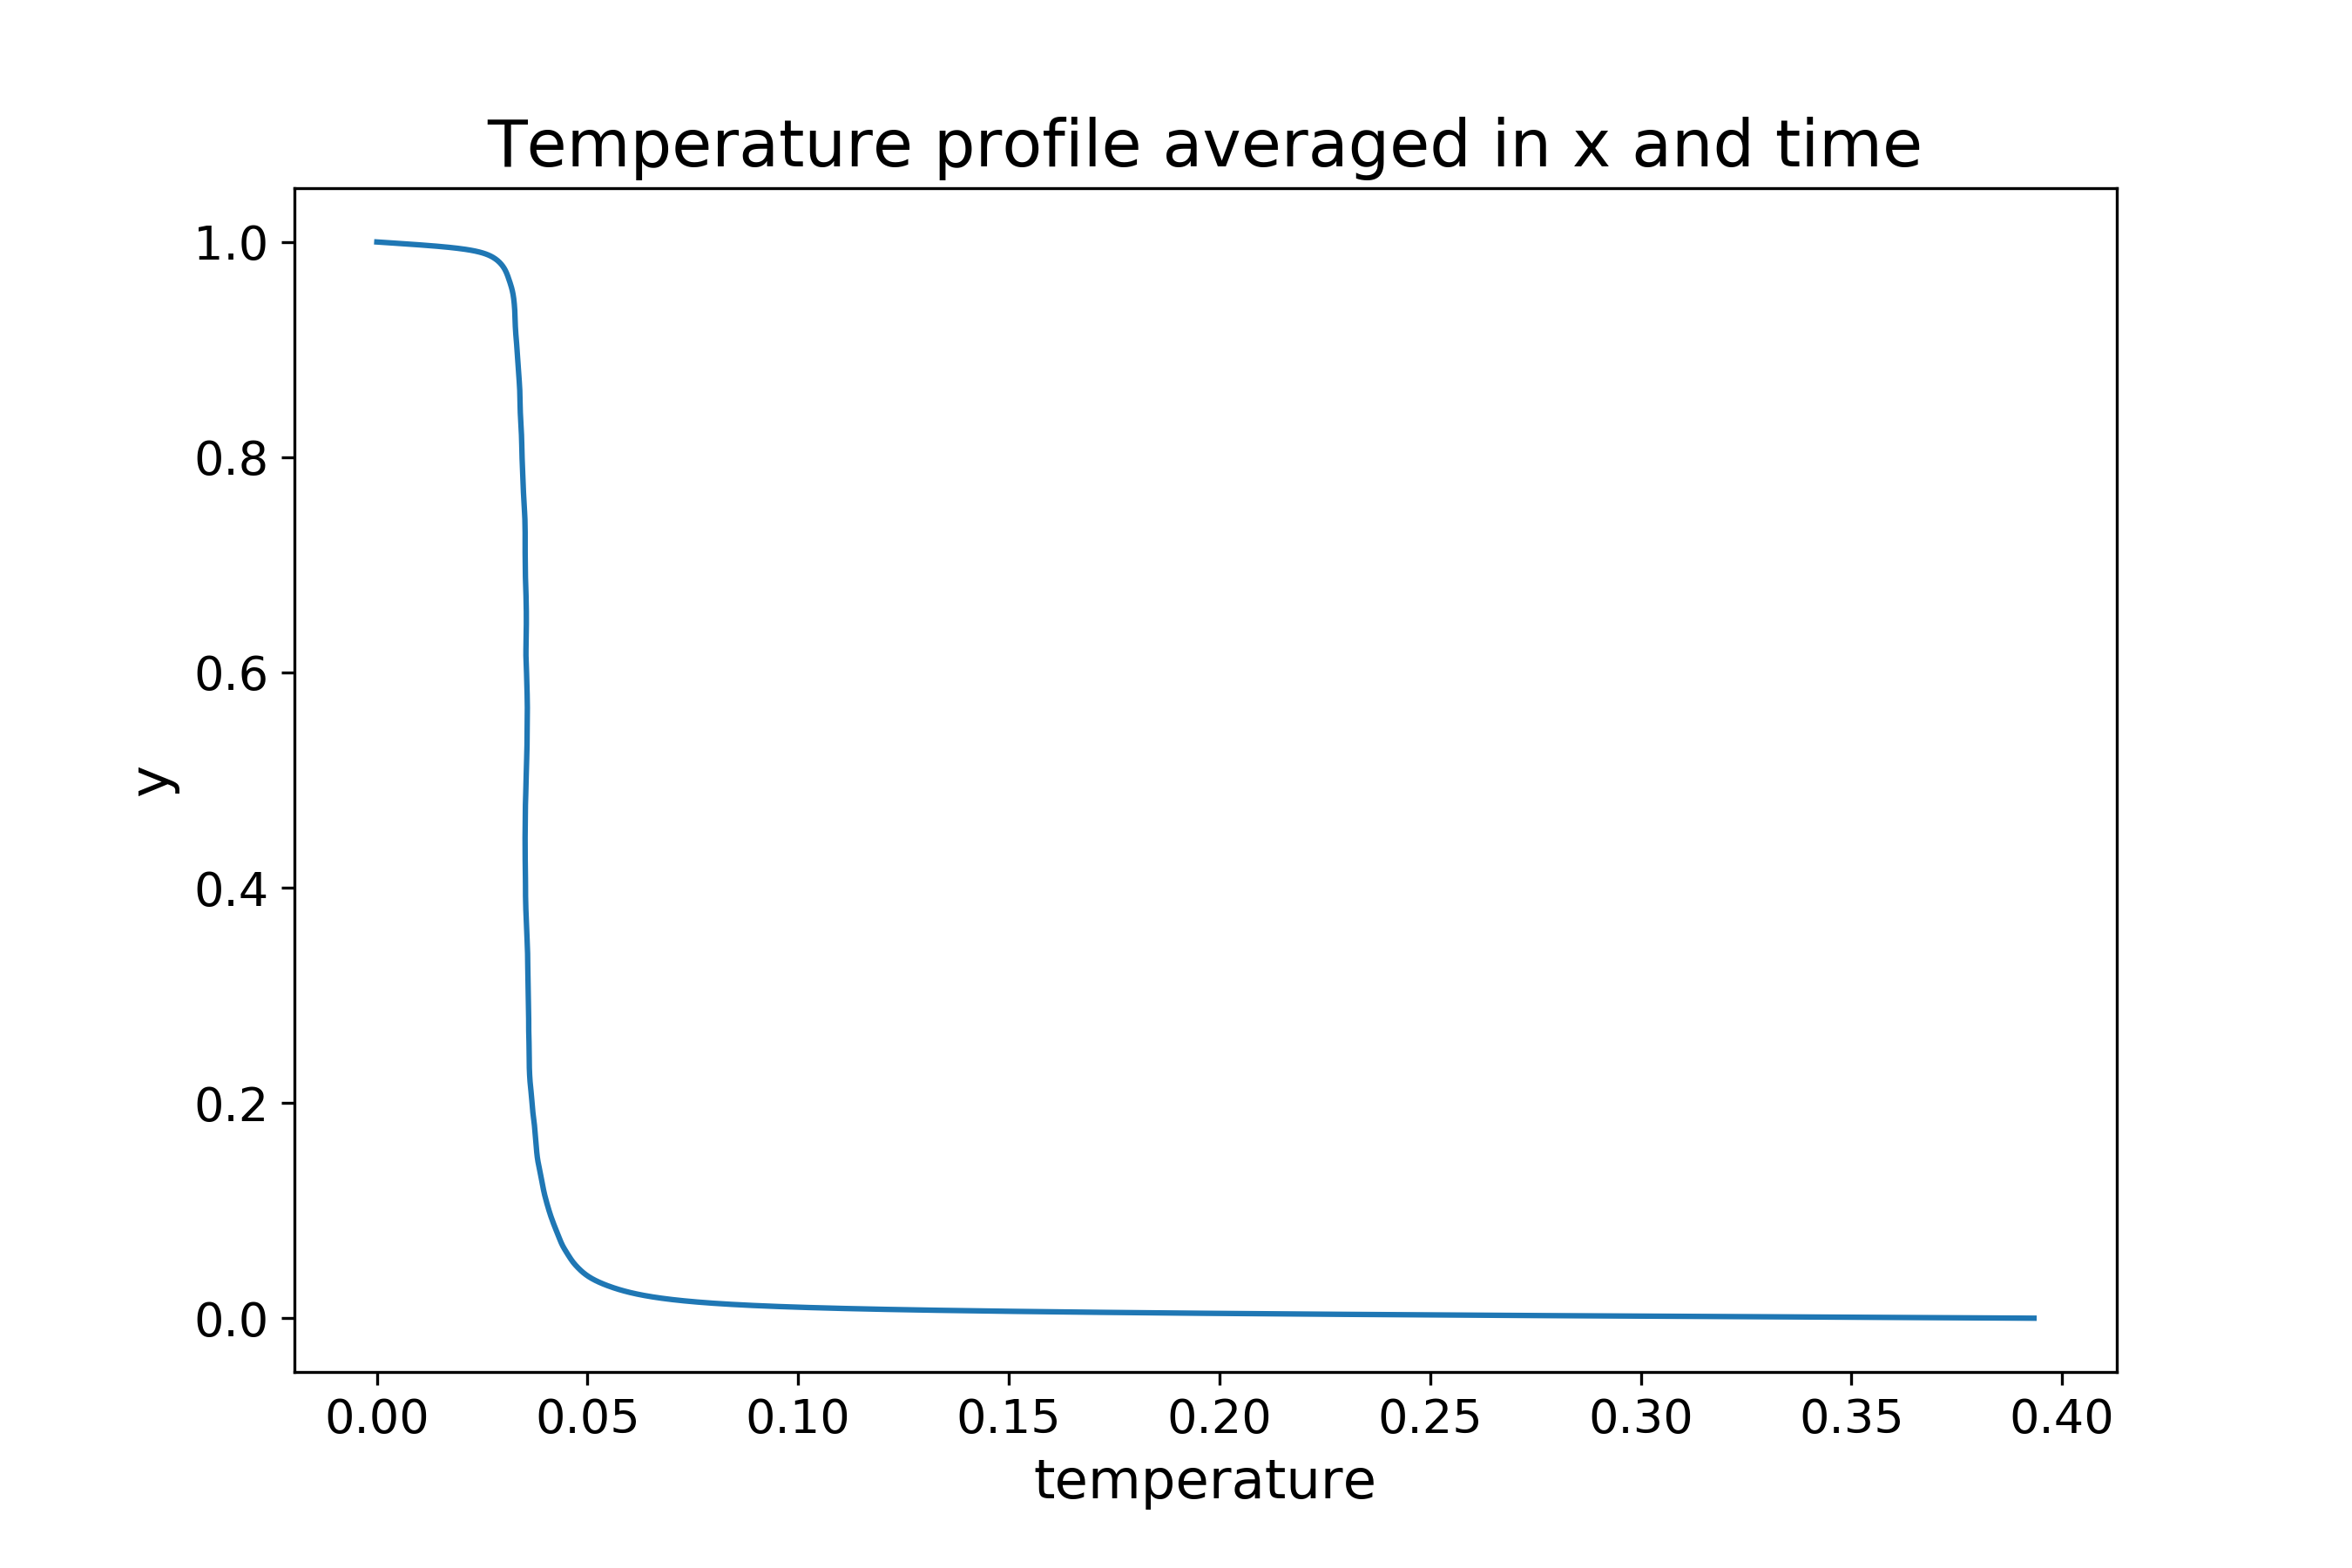
\includegraphics[scale=0.5]{temperature_y}
\centering
\caption{Temperature profile T(y) (averaged over x and t)}
\end{figure}

The average profile shows the temperature gradient but not the dynamics of the system. To show the time evolution, we plot the instant temperature profile at different time slots, as available in the video in the slides. Here only plots the last time frame. It shows a step-function-like front that keeps moving to the right (i.e. temperature increases). If the simulation continues, the "front" of the profile will finally reach $T=0.5$, which is the average of bottom and top temperature.

\begin{figure}[H]
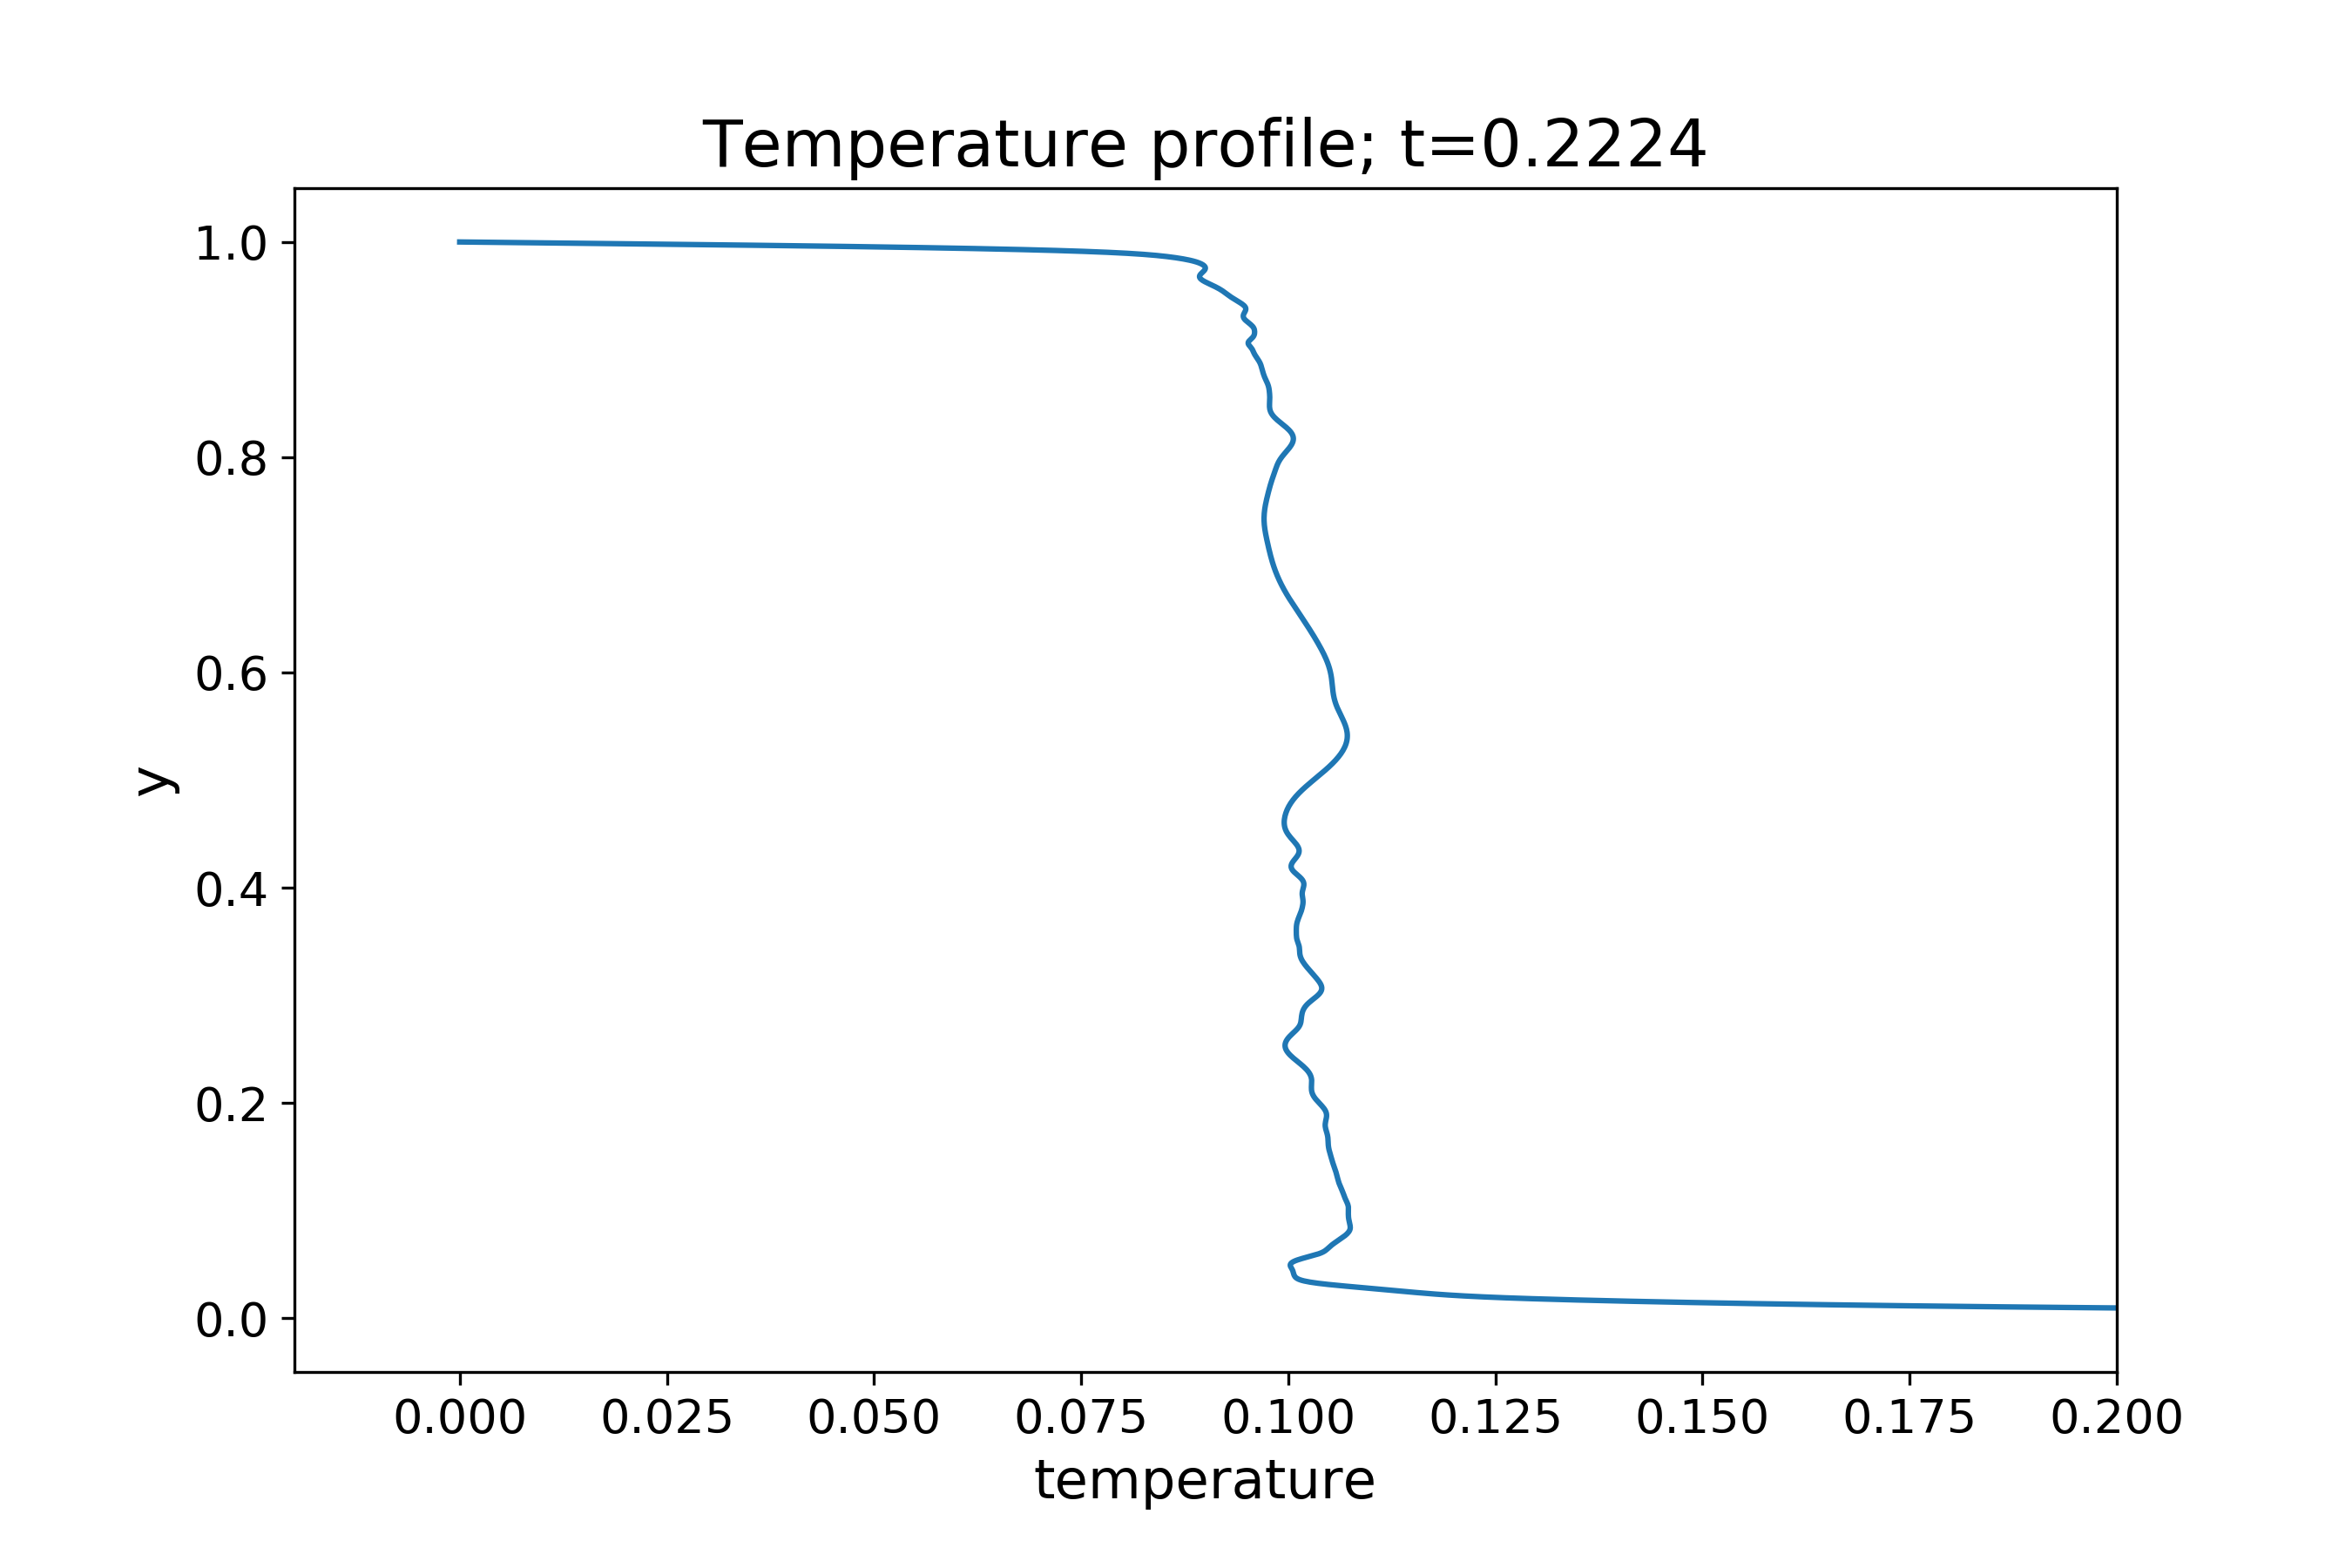
\includegraphics[scale=0.5]{profile_frame_224}
\centering
\caption{Temperature profile T(y) (averaged over x) at a single time frame. The "front" keeps moving to the right.}
\end{figure}

We can also put the profiles (averaged over x) together into one figure, with the x-axis indicating time evolution. 

\begin{figure}[H]
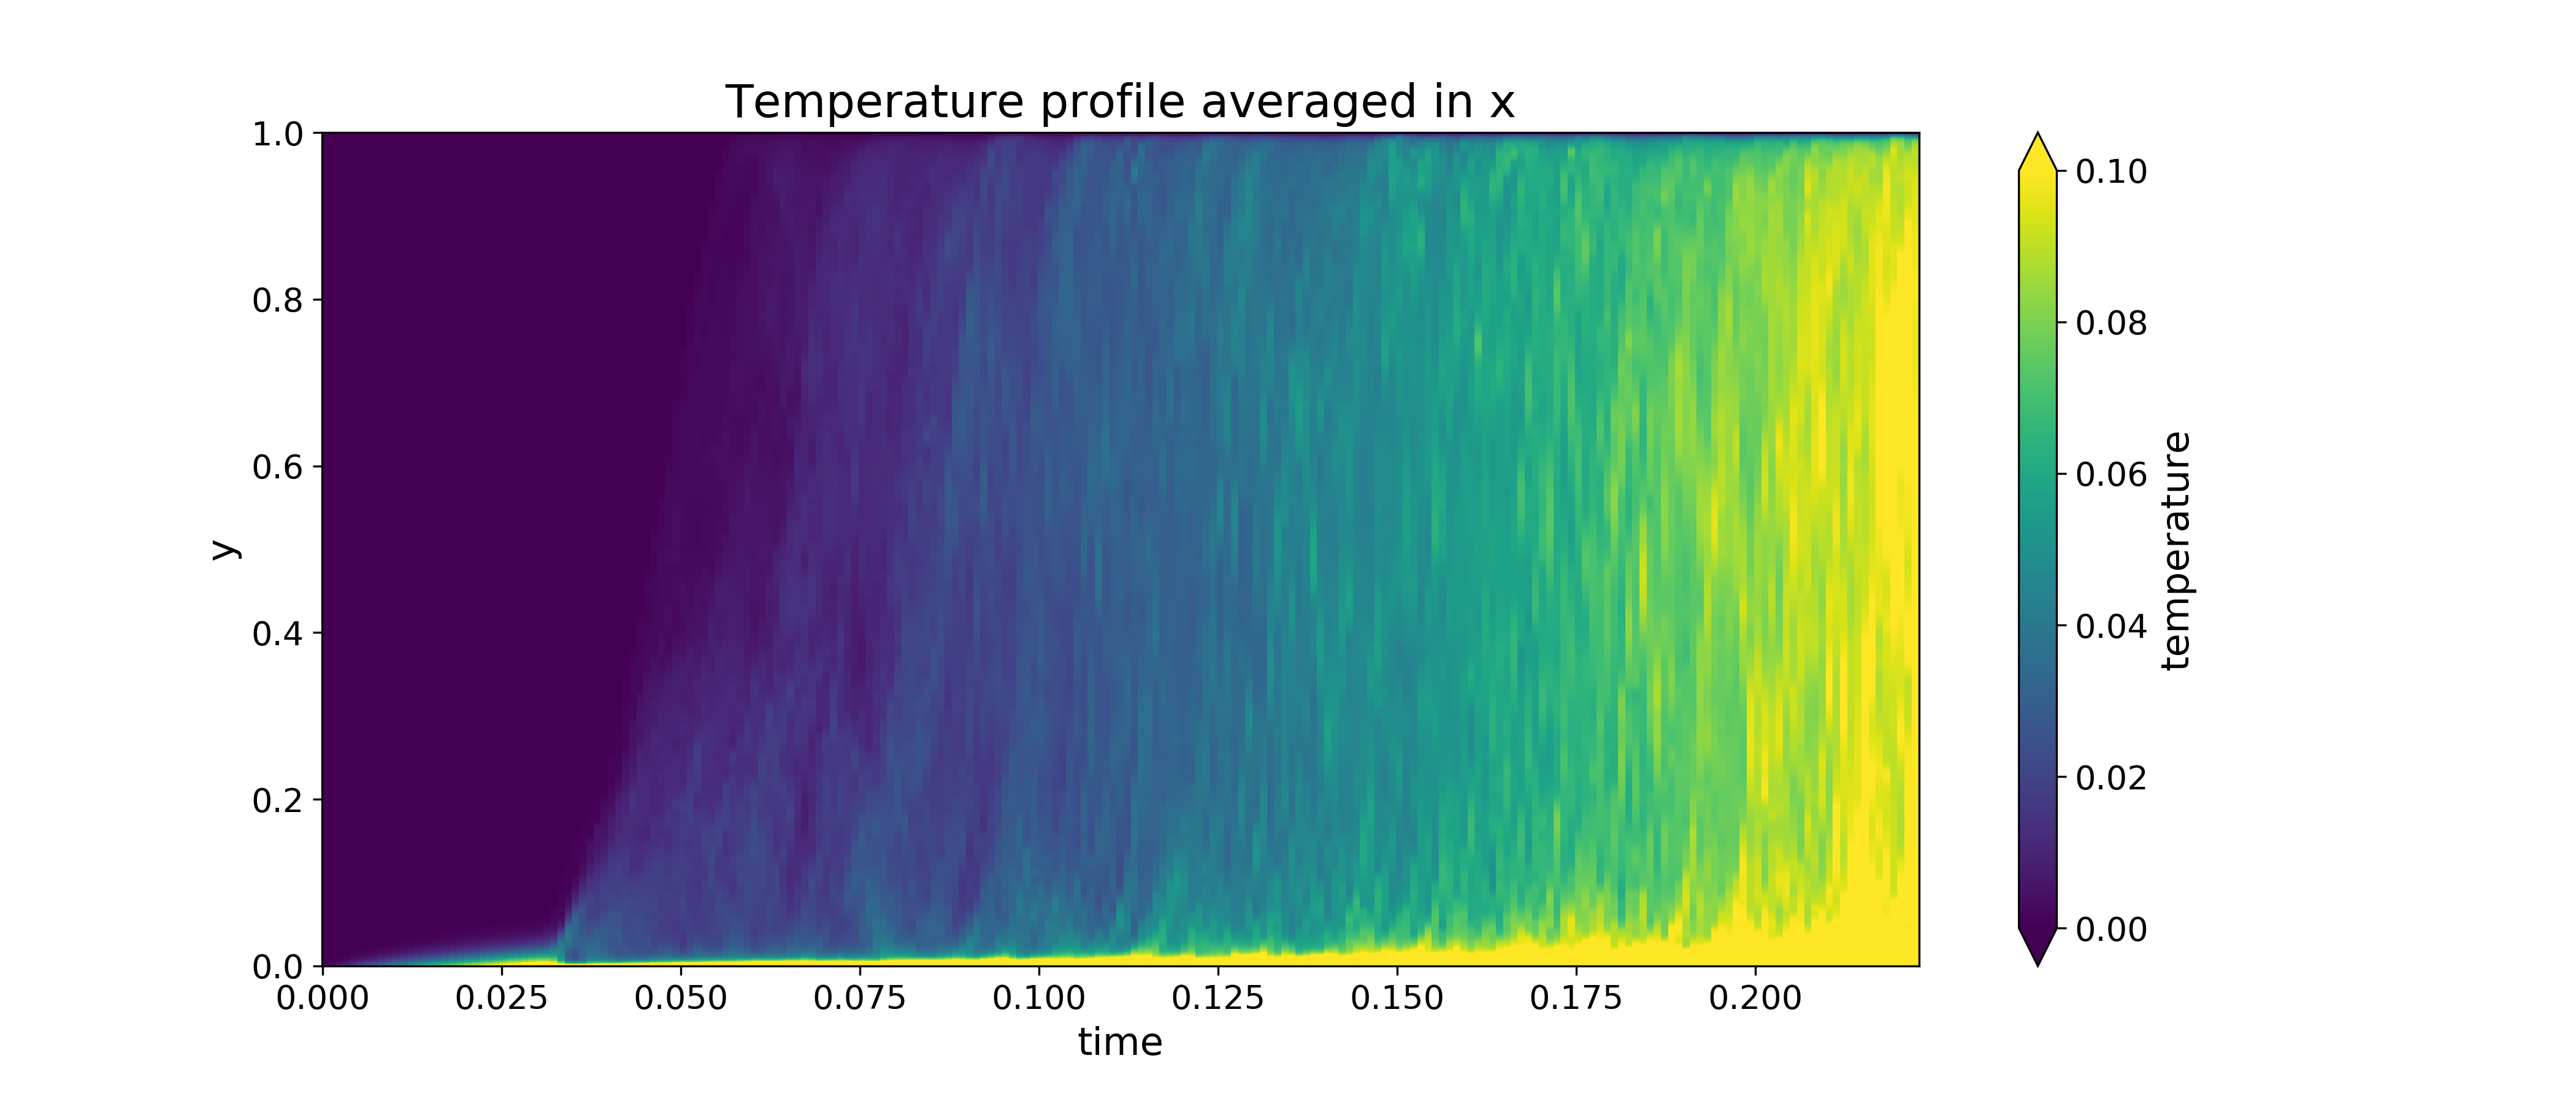
\includegraphics[scale=0.5]{temperature_y_time}
\centering
\caption{Temperature profile T(y, t) (averaged over x, change with time)}
\end{figure}

\subsubsection{Boundary condition}

The boundary condition $T(y=0)$ starts with 0 and gradually reaches 1. This is consistent with the input XML file. Given our relatively short simulation period, the bottom temperature at the last time step is still far from the steady state $T=1$.

\begin{figure}[H]
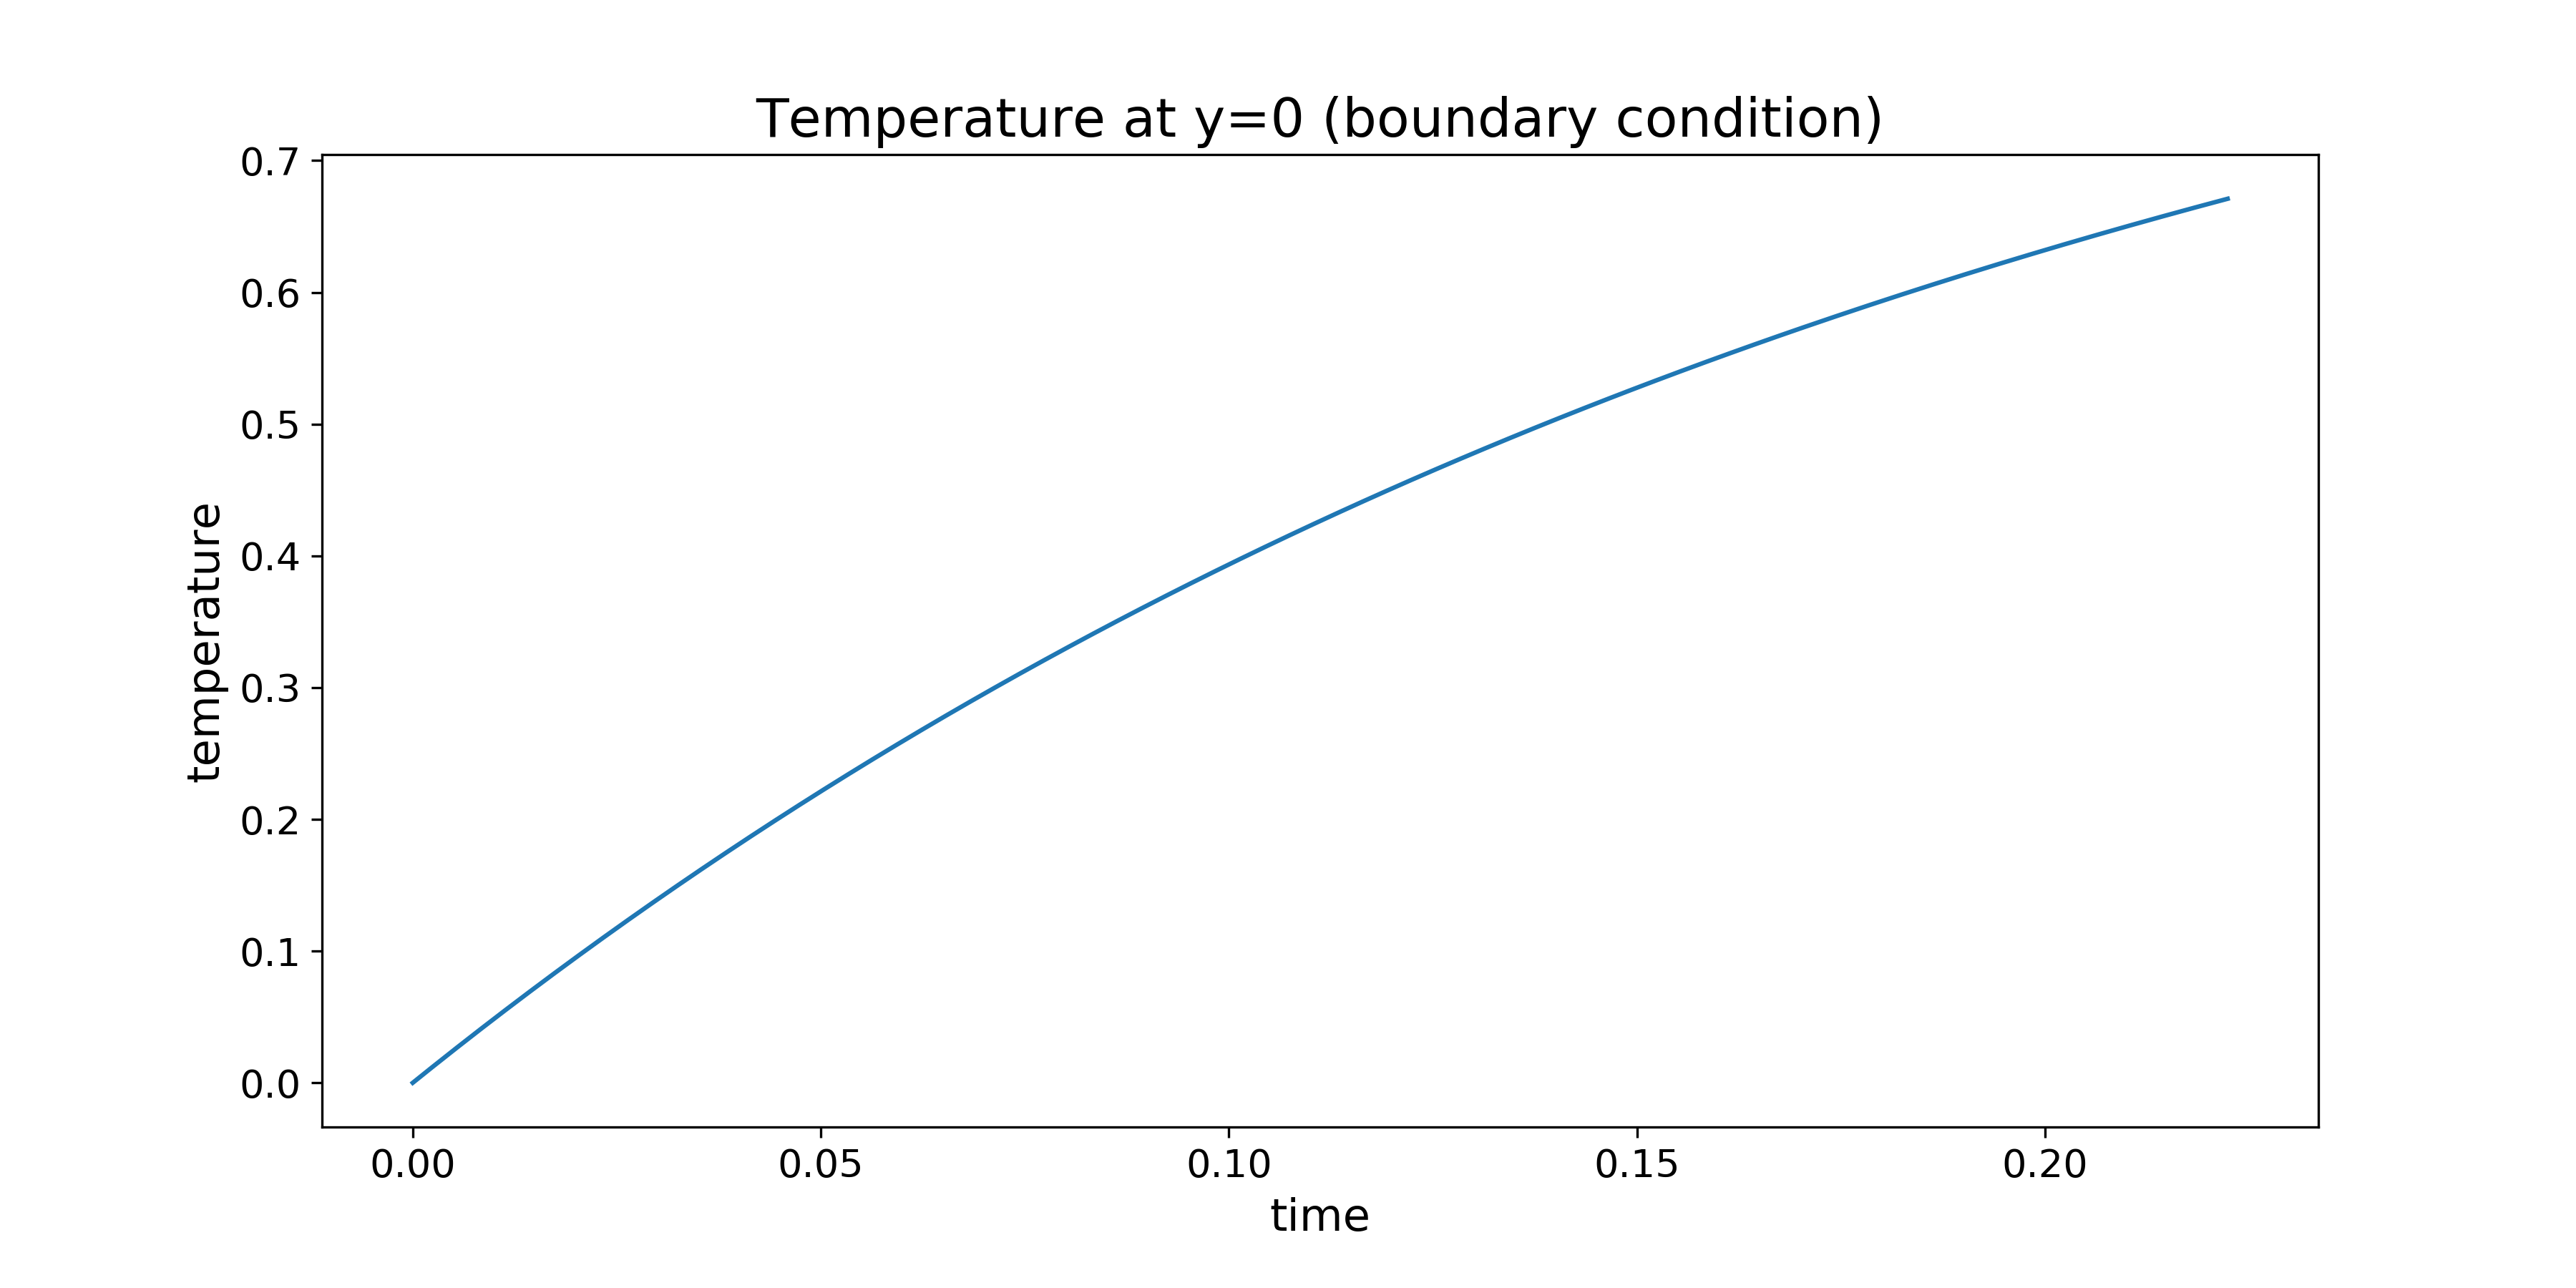
\includegraphics[scale=0.5]{y_bottom}
\centering
\caption{Boundary condition T(y=0)}
\end{figure}

\subsection{Schlieren visualization}

We then compute the Schlieren field from the temperature, using the formula:

\begin{align}
Sch = exp(-k\frac{|\nabla T|}{max(|\nabla T|)})
\end{align}

To get rich visualizations, we use a relatively large $k=50$. With small $k$, most areas will be dark (values close to 1).

\begin{figure}[H]
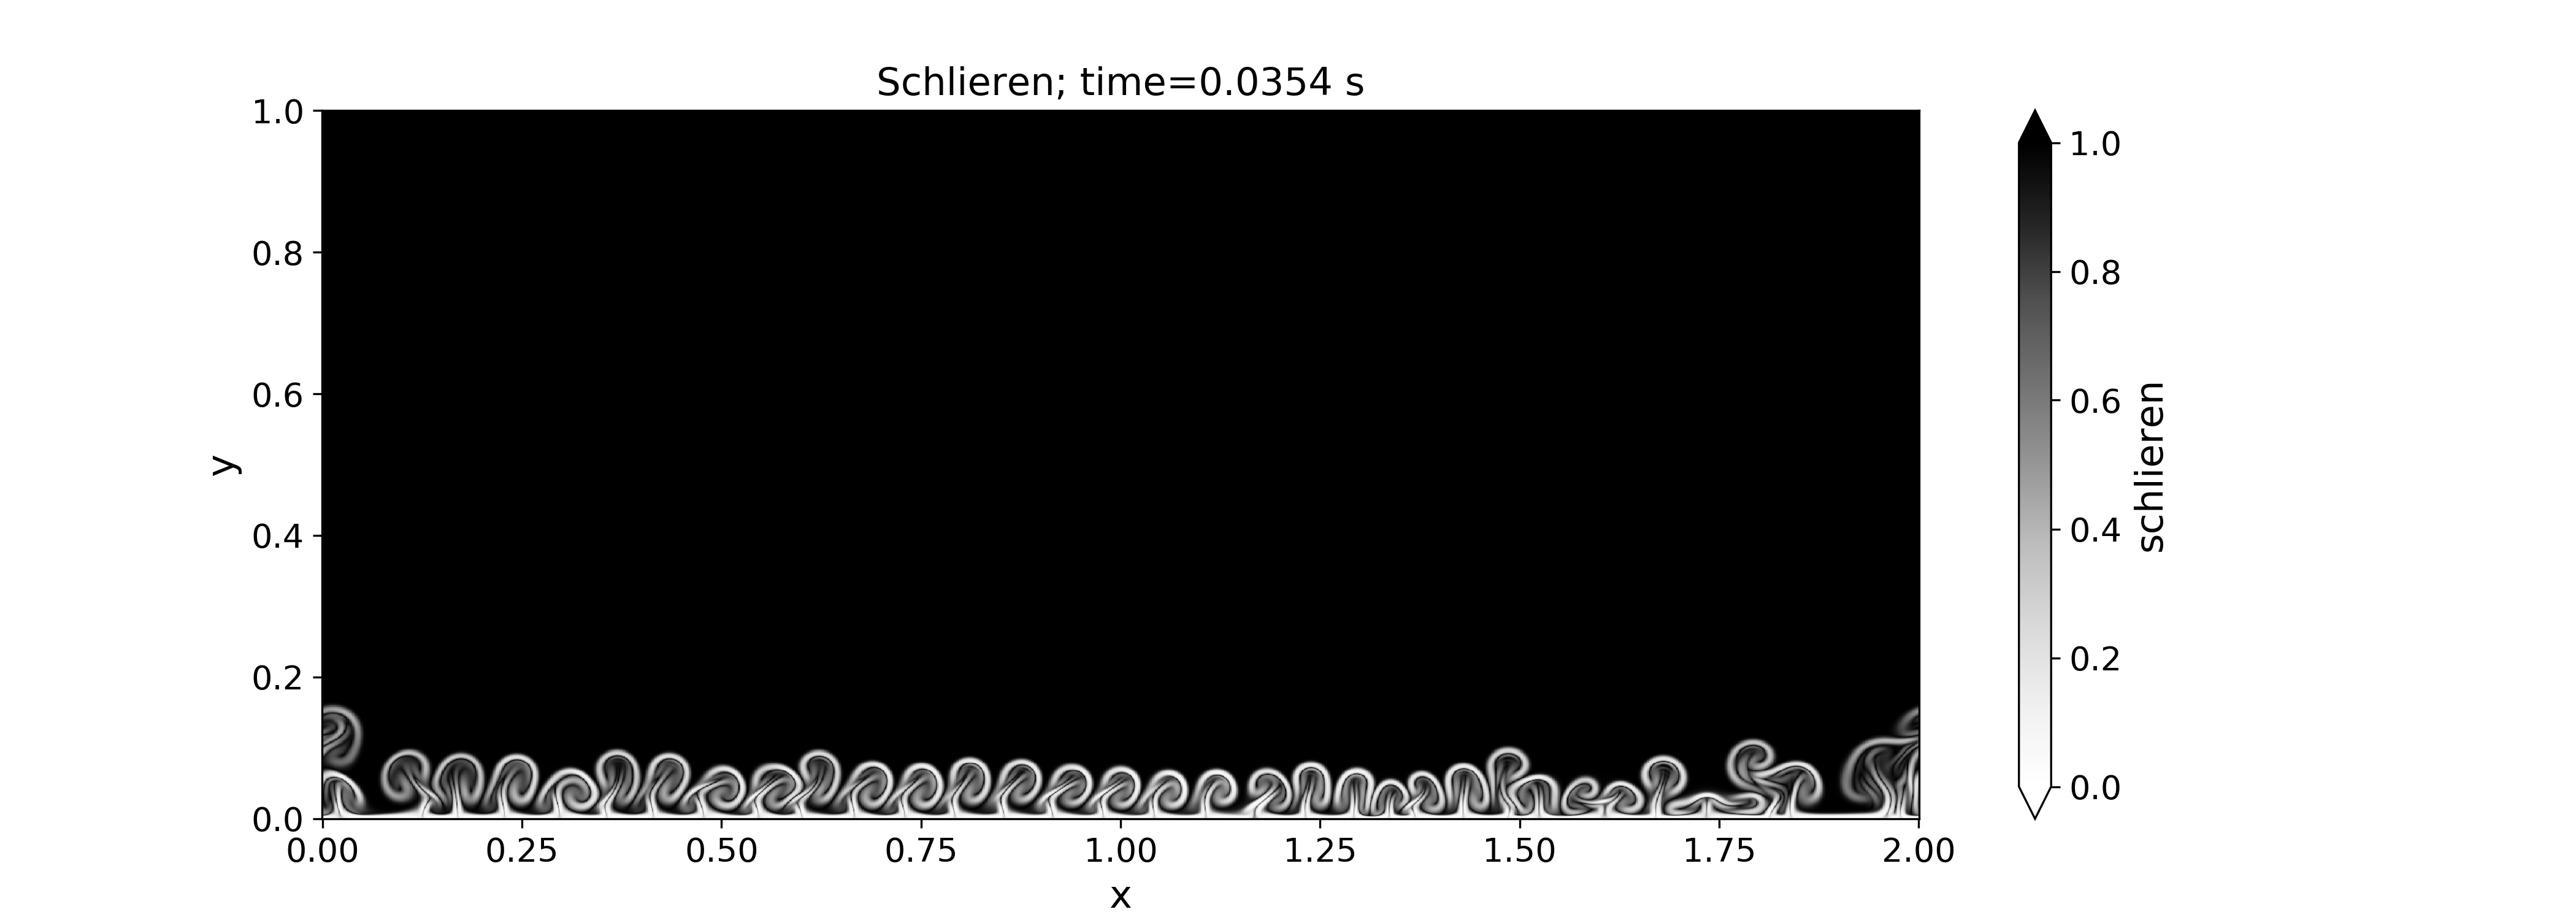
\includegraphics[scale=0.5]{sch_k50_frame_037}
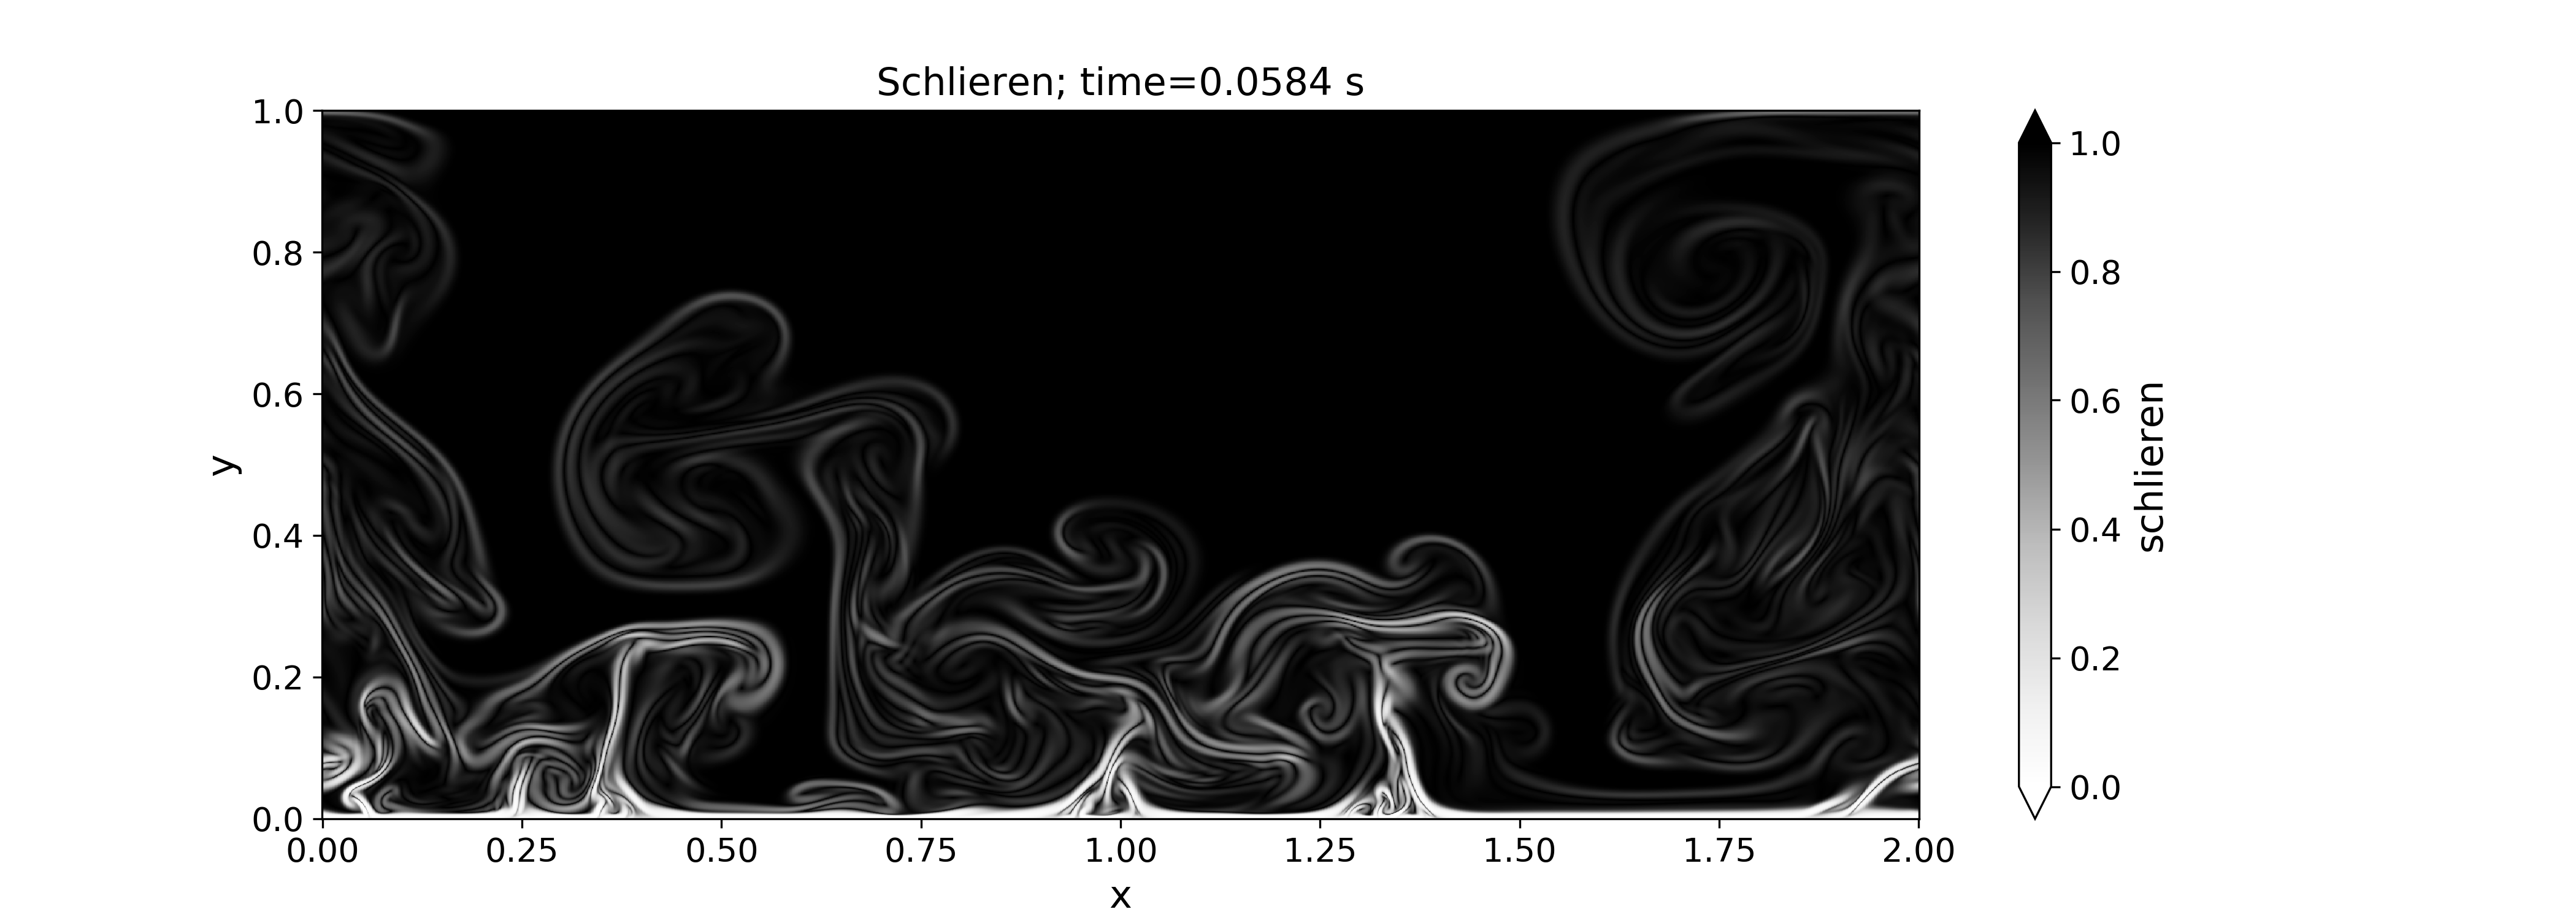
\includegraphics[scale=0.5]{sch_k50_frame_060}
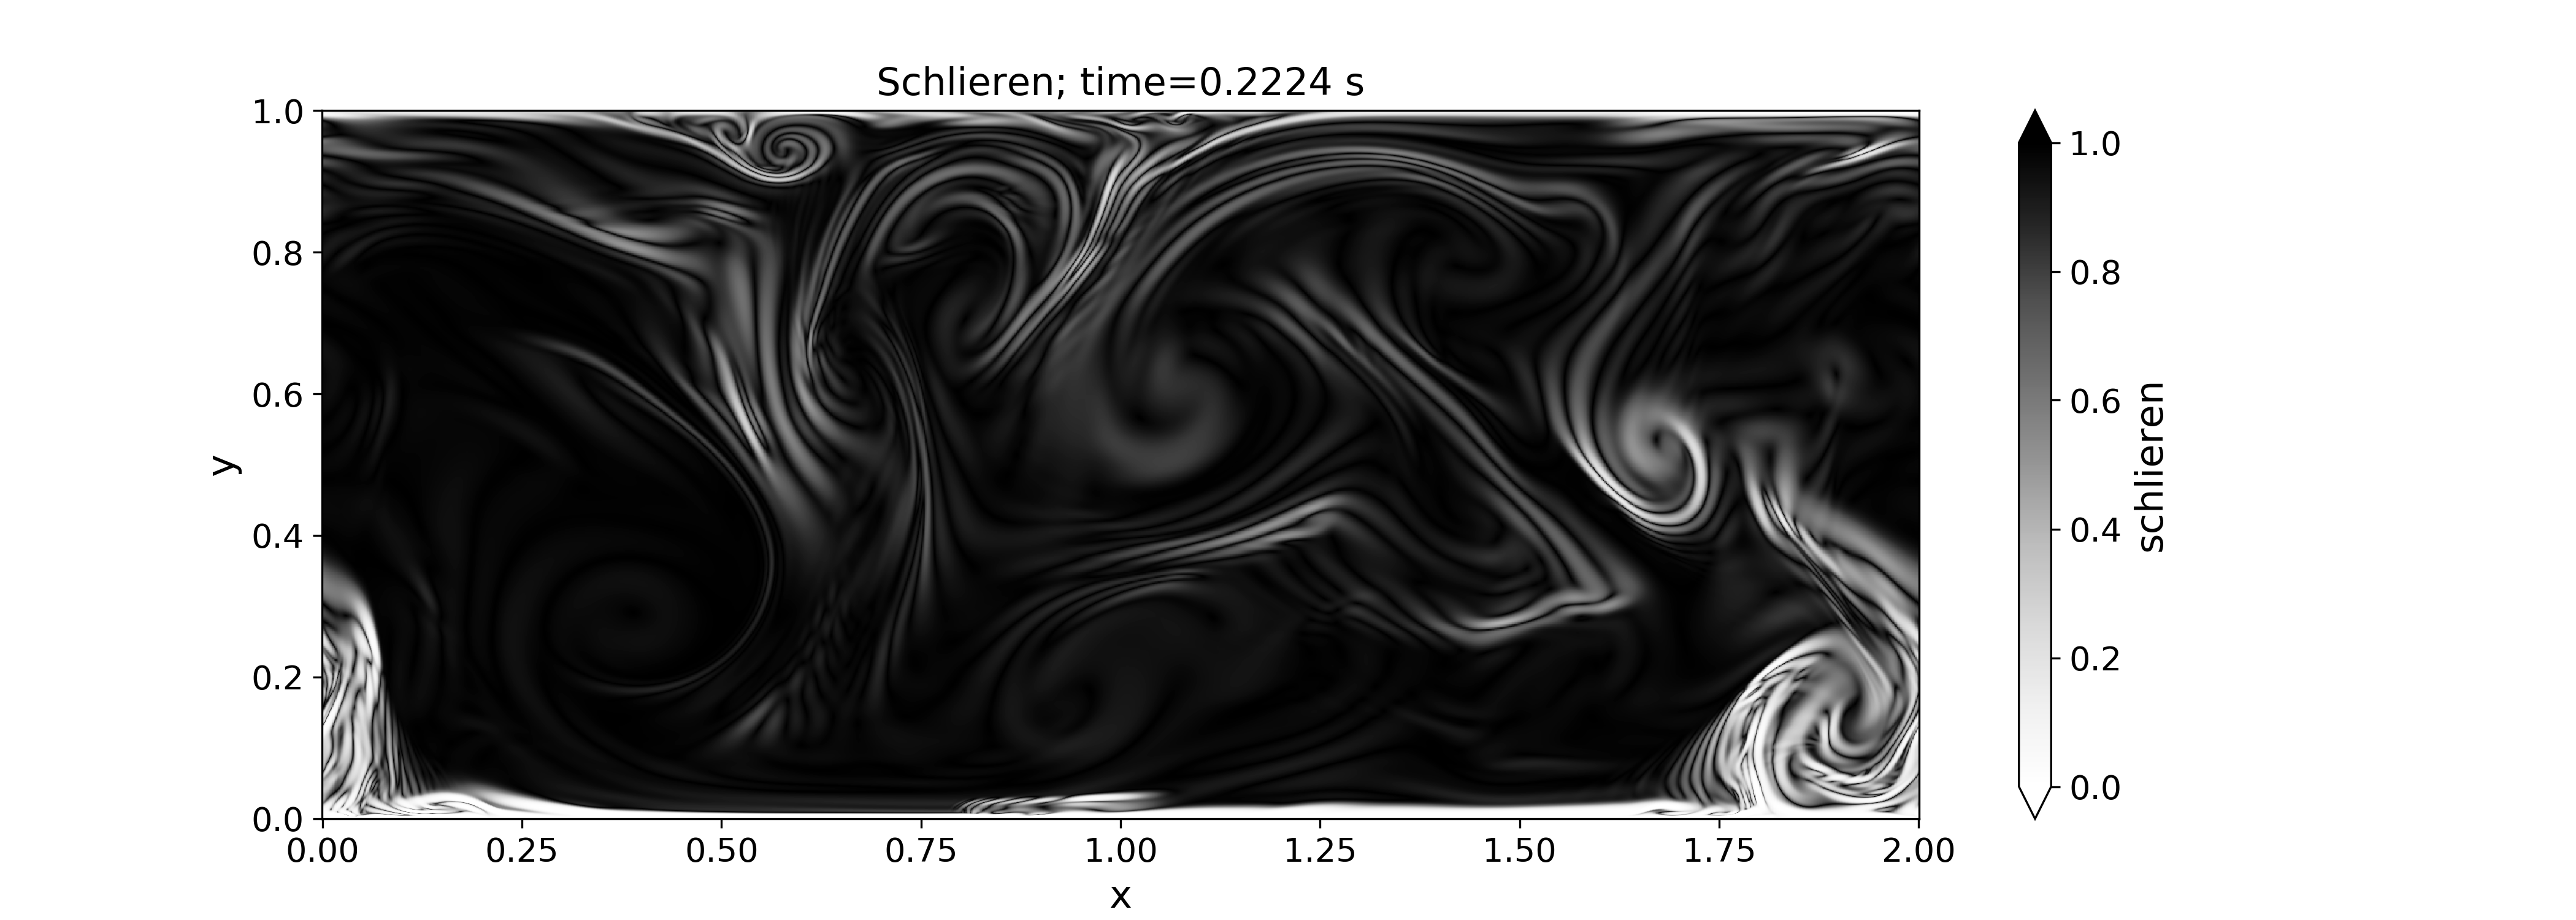
\includegraphics[scale=0.5]{sch_k50_frame_224}
\centering
\caption{Schlieren visualization with k=50}
\end{figure}

\begin{figure}[H]
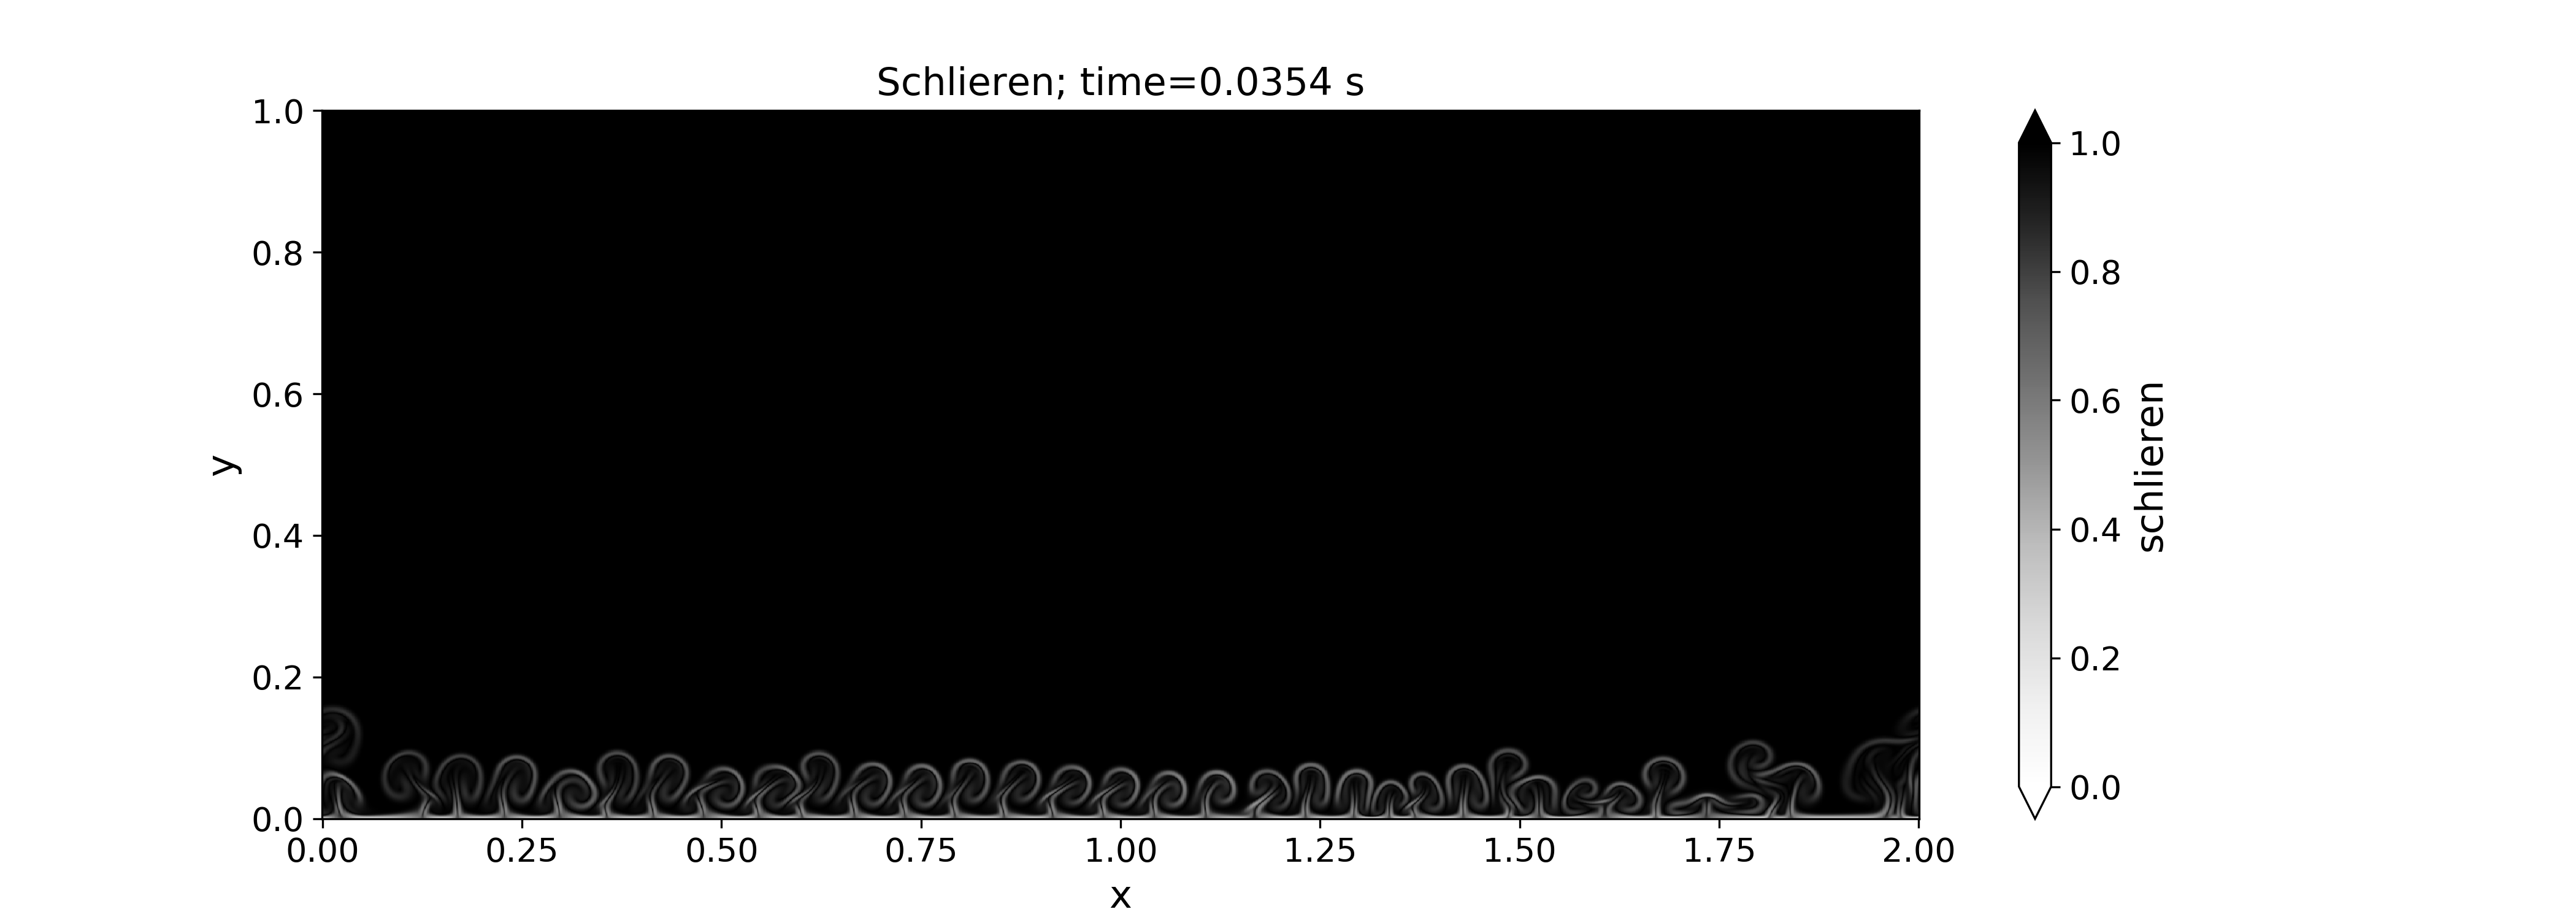
\includegraphics[scale=0.5]{sch_k10_frame_037}
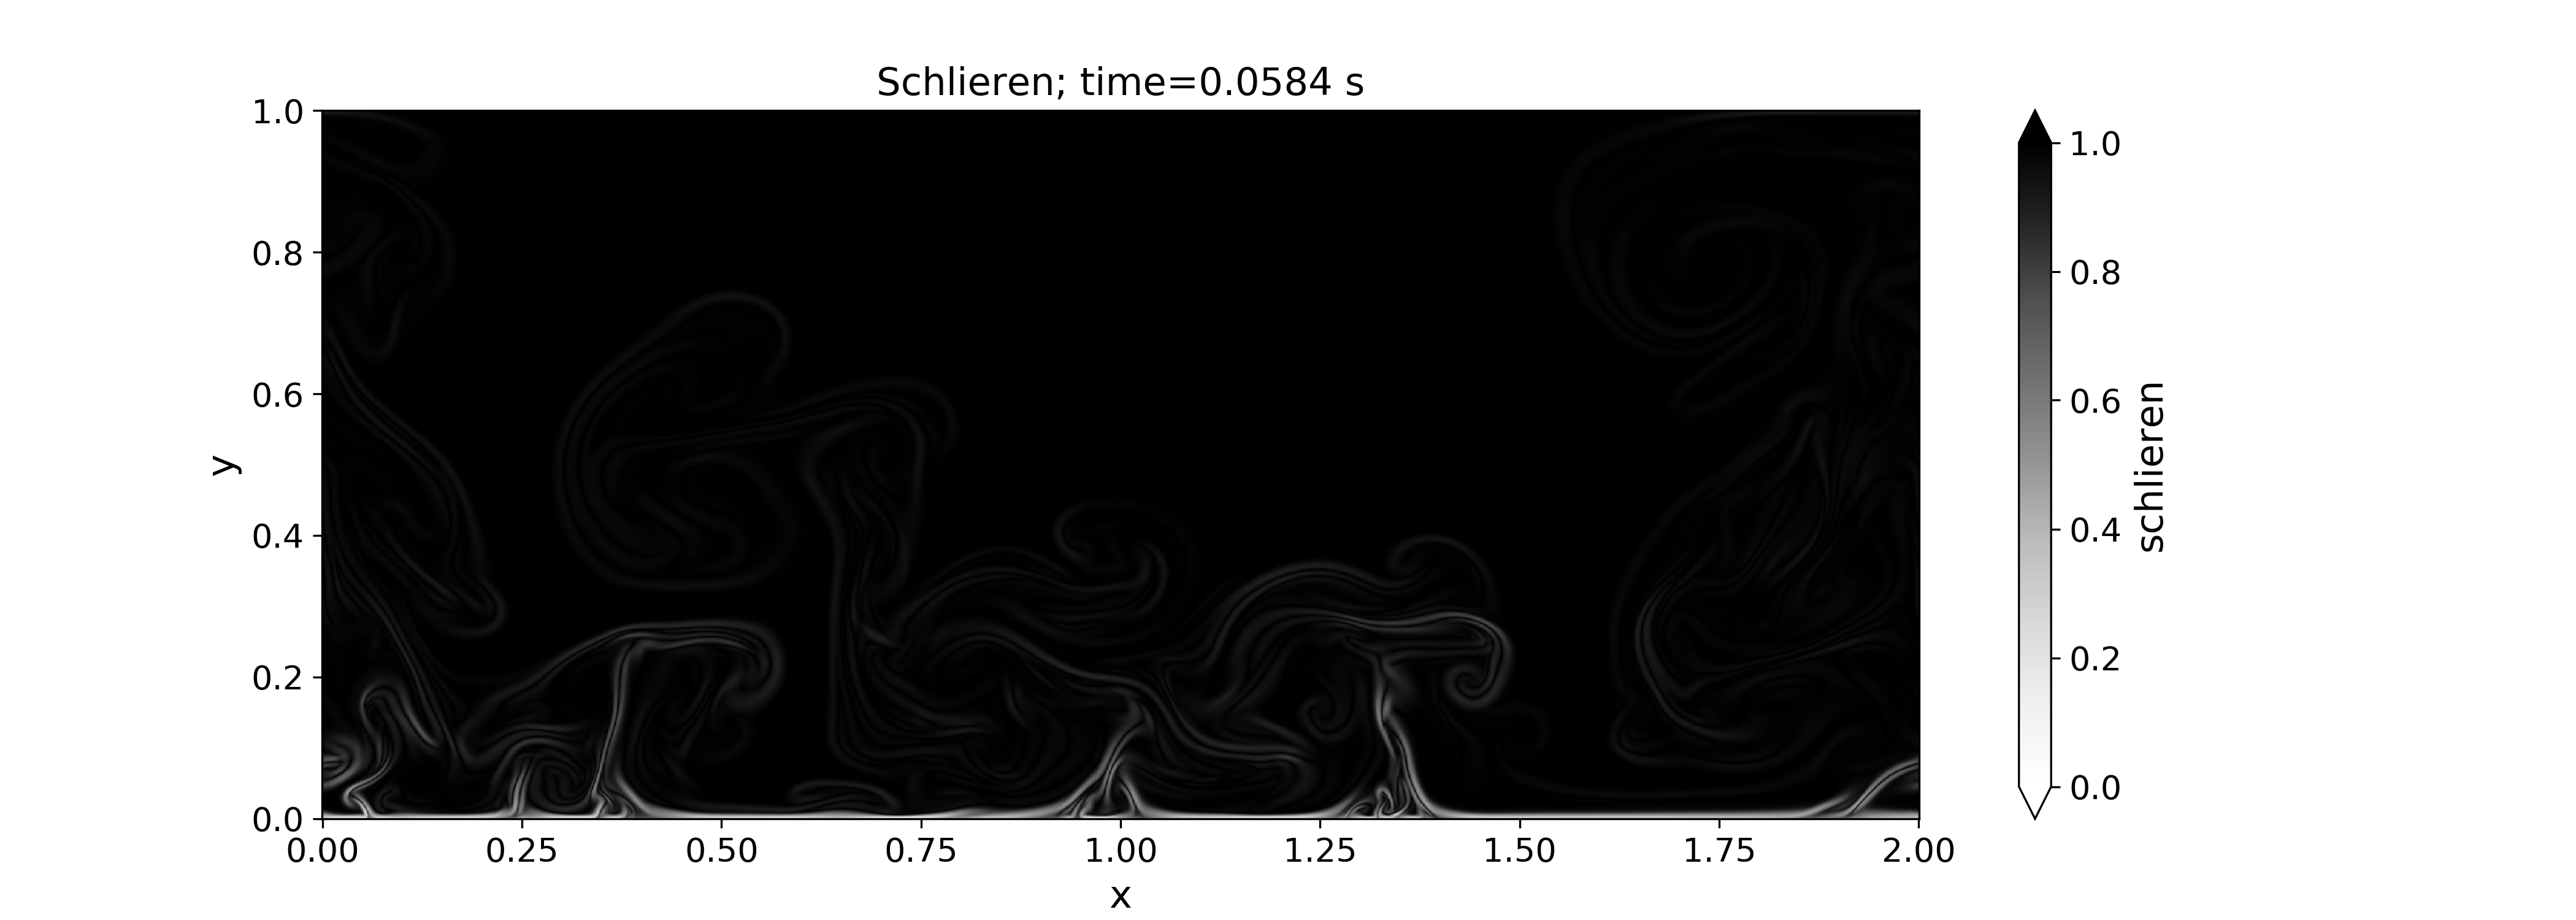
\includegraphics[scale=0.5]{sch_k10_frame_060}
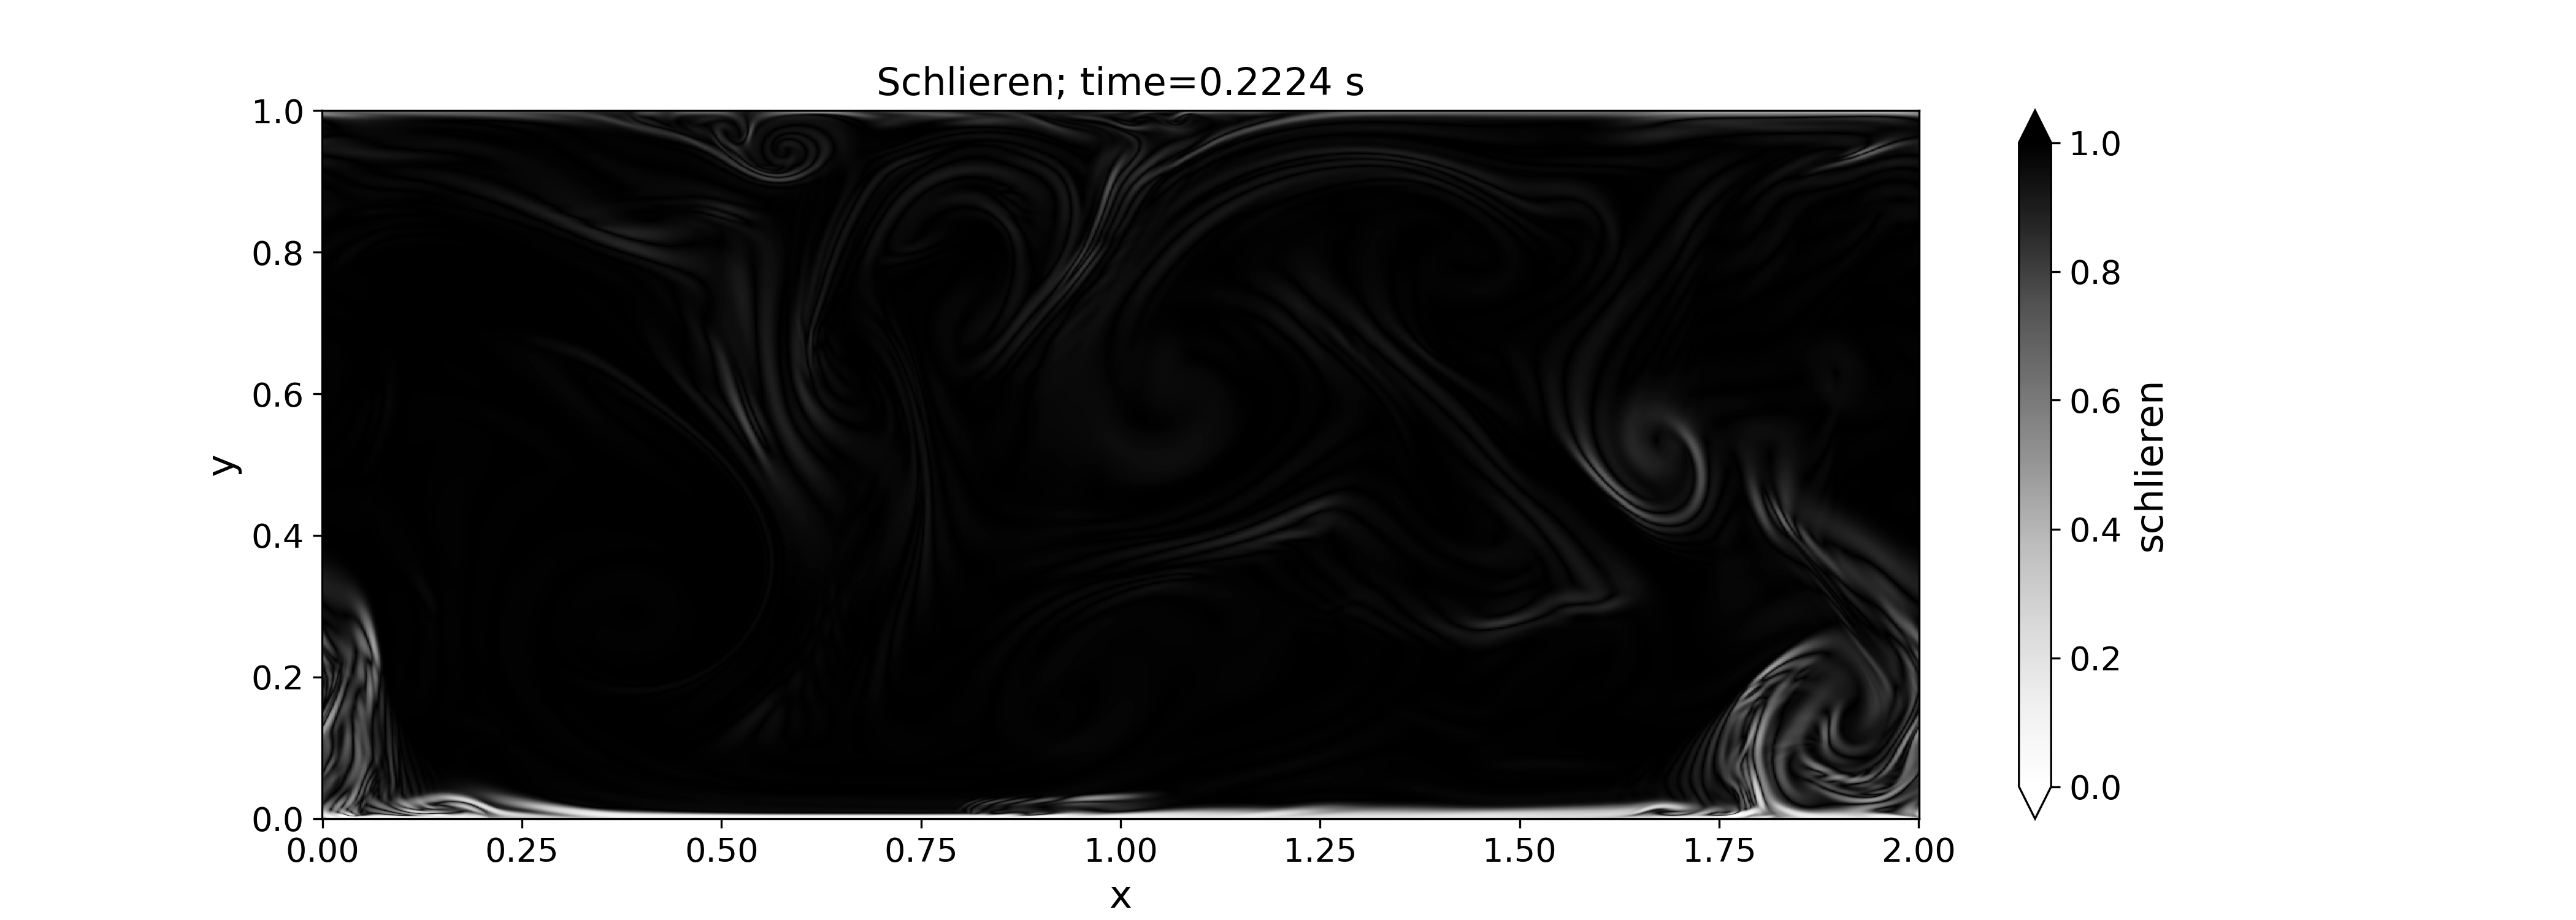
\includegraphics[scale=0.5]{sch_k10_frame_224}
\centering
\caption{Schlieren visualization with k=10}
\end{figure}

\subsection{Nusselt number}

Finally we compute the Nusselt number which indicates the ratio of convective heat transfer to conductive heat transfer. After $t > 0.005$ the Nusselt number settles around 130. Its magnitude is consistent with existing literature [2].

\begin{figure}[H]
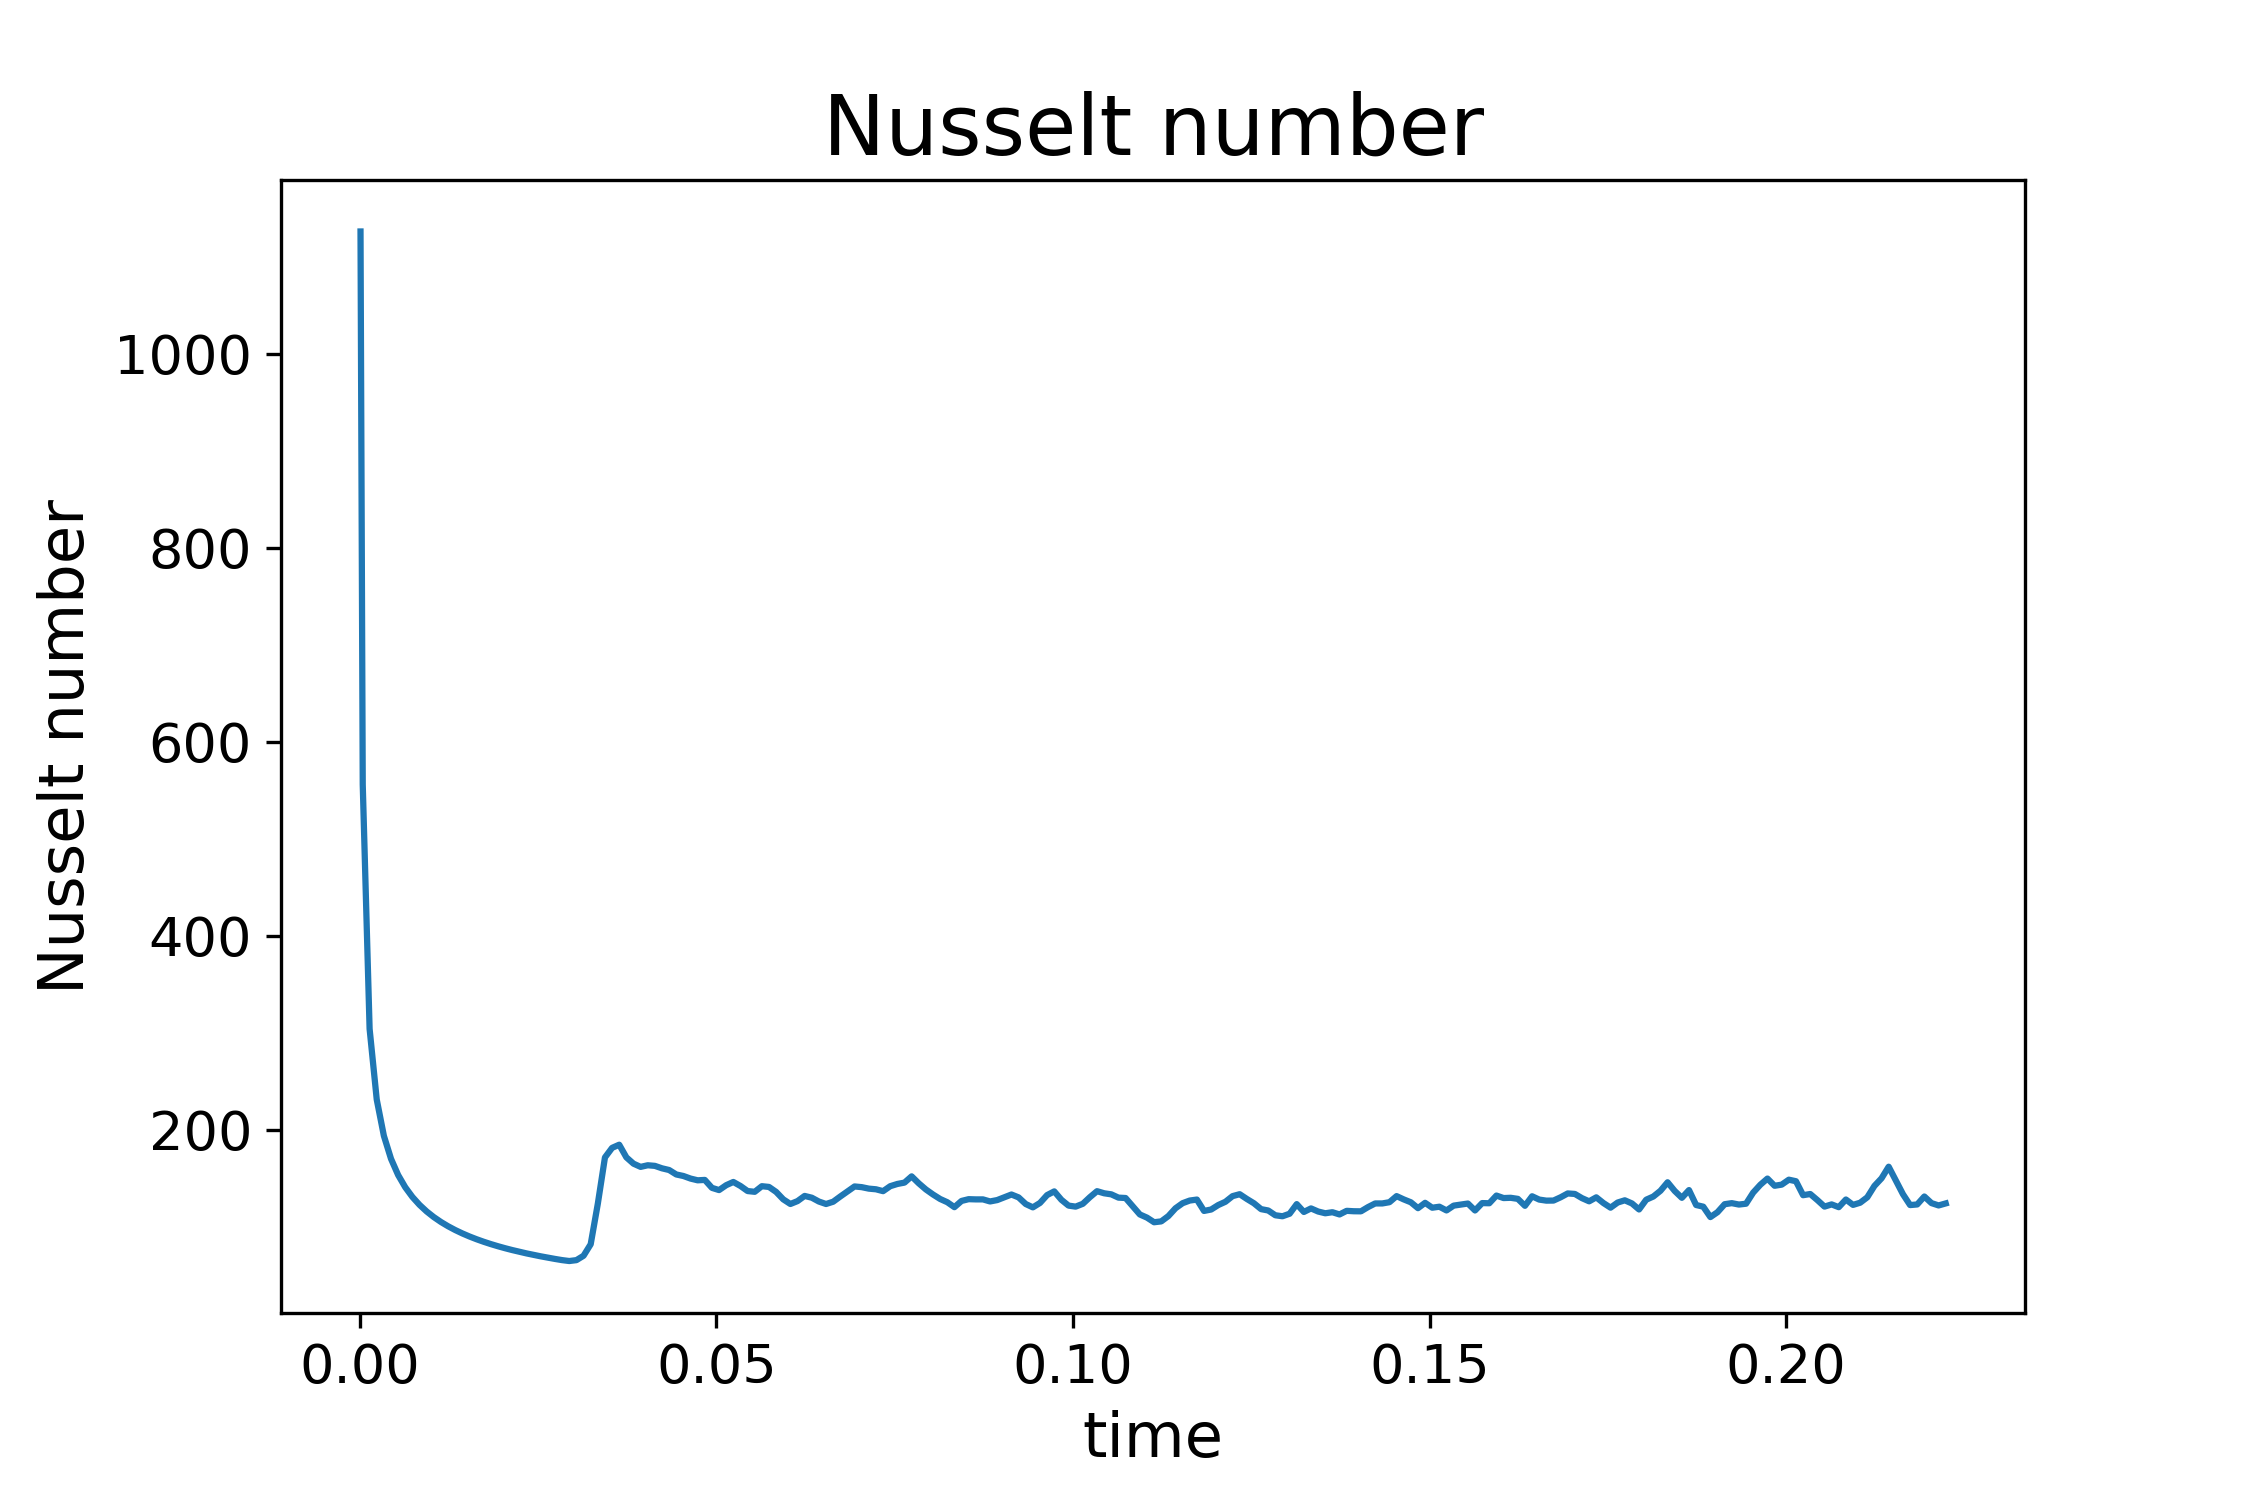
\includegraphics[scale=0.5]{Nusselt_number}
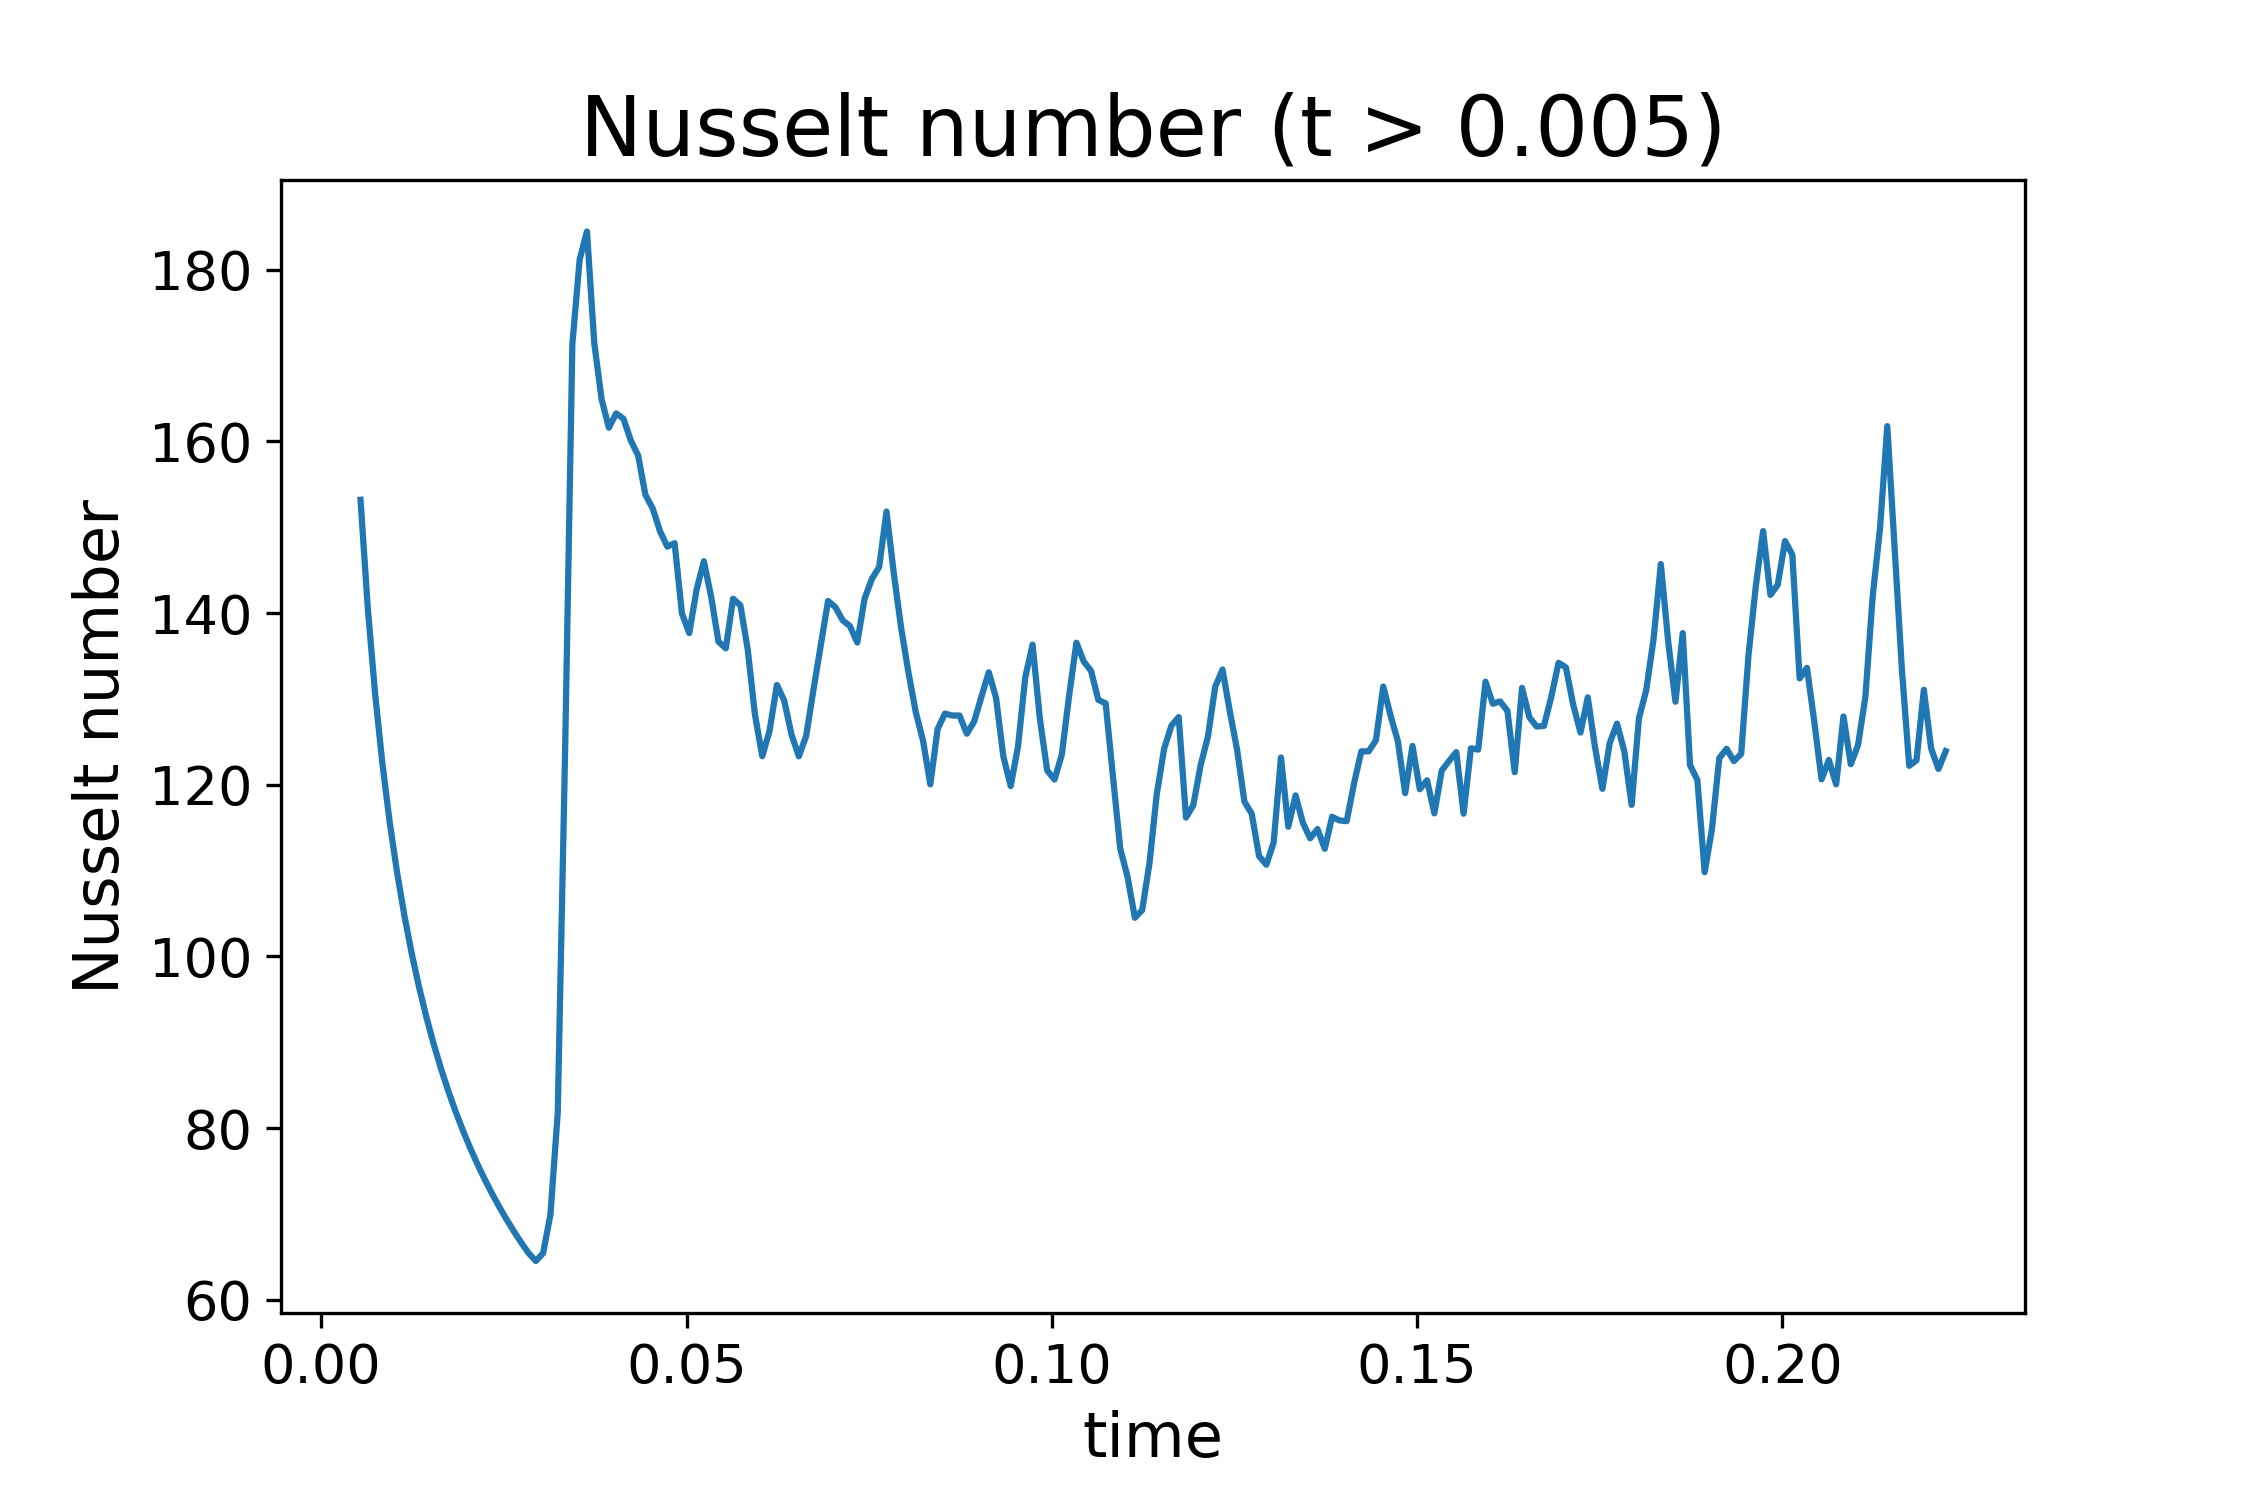
\includegraphics[scale=0.5]{Nusselt_number_truncate}
\centering
\caption{Nusselt number (time-dependent)}
\end{figure}


\section{Conclusion and Future Work}
In this work, we studied the Rayleigh-Bénard convection of $Ra=10^{10}$, $Pr=1$ through numerical simulation on a high performance computing platform. From the simulation results, we provided a thorough analysis of the temperature distribution over time. We observed the formation and mixing of plumes in RBC, as well as natural eddies formed by changes in density. The time dependent temperature profile provided a more intuitive description of the mixing process. In addition, the Nusselt number of the system was calculated as a function of time. Towards the thermal equilibrium, the Nusselt number converged to approximately 120. A value often described as identifying what some researchers describe as turbulent flow. 

Due to limited computational resources, the simulation performed in this work did not arrive at a physical time which could be considered long enough. That is, although much occurred within the observed timeframe, much is left to be said about the dynamic flow which will occur after. For the future work, we envision running the simulation on more CPUs with longer a longer timeframe. Another interesting work would be to model thermal within other objects and environments, a common research topic in various fields.


\bibliographystyle{unsrt}  
%\bibliography{references}  %%% Remove comment to use the external .bib file (using bibtex).
%%% and comment out the ``thebibliography'' section.


%%% Comment out this section when you \bibliography{references} is enabled.
\begin{thebibliography}{1}

\bibitem{cattle}
Bruce, J. M. 
\newblock Natural convection through openings and its application to cattle building ventilation. 
\newblock In {\em Journal of Agricultural Engineering Research}, 23(2), 151-167.

\bibitem{cattle}
Zhu, Xiaojue, et al.
\newblock Transition to the ultimate regime in two-dimensional Rayleigh-Bénard convection.
\newblock In {\em Physical review letters}, 120.14 (2018): 144502.

\end{thebibliography}


\end{document}
